\documentclass[11pt, letterpaper]{article}

% Fonts and Encoding
\usepackage[utf8]{inputenc}
\usepackage[T1]{fontenc}
\usepackage{lmodern} % High-quality Latin Modern vector font

% Math and Symbols
\usepackage{amsmath, amssymb, amsthm, amsfonts, mathrsfs, mathtools}

% Layout and Geometry
\usepackage{geometry}
\geometry{letterpaper, margin=1in}
\setlength{\parindent}{0pt}
\setlength{\parskip}{0.6em}

% Formatting and Graphics
\usepackage{graphicx, xcolor, enumitem, booktabs, array, tabularx}

% TikZ for Illustrations
\usepackage{tikz}
\usetikzlibrary{arrows.meta, positioning, shapes.geometric, calc, backgrounds, matrix}

% Clickable Links and TOC
\usepackage{hyperref}
\hypersetup{
    colorlinks=true,
    linkcolor=blue,
    filecolor=magenta,      
    urlcolor=cyan,
    pdftitle={Constrained Optimization of Quadratic Forms},
}

% Theorem Environments
\newtheorem{theorem}{Theorem}[section]
\newtheorem{lemma}[theorem]{Lemma}
\newtheorem{proposition}[theorem]{Proposition}
\newtheorem{corollary}[theorem]{Corollary}
\theoremstyle{definition}
\newtheorem{definition}{Definition}[section]
\newtheorem{axiom}{Axiom}[section]
\newtheorem{example}{Example}[section]
\theoremstyle{remark}
\newtheorem{remark}{Remark}[section]

% Custom Commands (Enforced standard notation)
\newcommand{\R}{\mathbb{R}}
\newcommand{\N}{\mathbb{N}}
\newcommand{\Z}{\mathbb{Z}}
\newcommand{\Q}{\mathbb{Q}}
\newcommand{\E}{\mathbb{E}}
\newcommand{\Prob}{\mathbb{P}}
\newcommand{\F}{\mathcal{F}}

\title{\textbf{Mastery Study Guide: Section 7.3 Constrained Optimization}}
\author{Tashfeen Omran}
\date{\today}

\begin{document}

\maketitle
\tableofcontents
\newpage

% ============================================================================
% PART 1: COMPREHENSIVE INTRODUCTION, CONTEXT, AND PREREQUISITES
% ============================================================================
\section{Comprehensive Introduction, Context, and Prerequisites}

\subsection{Core Concepts}
In engineering, economics, statistics, and physical sciences, one frequently seeks to maximize or minimize a quadratic form $Q(\mathbf{x}) = \mathbf{x}^T A \mathbf{x}$ (where $A$ is an $n \times n$ real symmetric matrix) as $\mathbf{x}$ varies over a specified constraint set. Without constraints, a non-degenerate quadratic form is unbounded on $\mathbb{R}^n$ (scaling $\mathbf{x}$ by $c \to \infty$ scales $Q(c\mathbf{x}) = c^2 Q(\mathbf{x}) \to \pm \infty$). Therefore, meaningful optimization requires bounding the input vector $\mathbf{x}$.

The canonical and most fundamental constraint requires $\mathbf{x}$ to be a \textbf{unit vector} in $\mathbb{R}^n$. This unit-sphere constraint can be expressed in four completely equivalent ways:
\[
\|\mathbf{x}\| = 1, \qquad \|\mathbf{x}\|^2 = 1, \qquad \mathbf{x}^T \mathbf{x} = 1, \qquad x_1^2 + x_2^2 + \cdots + x_n^2 = 1.
\]
We define the minimum and maximum values of $Q(\mathbf{x}) = \mathbf{x}^T A \mathbf{x}$ on the unit sphere $S^{n-1} = \{\mathbf{x} \in \mathbb{R}^n : \|\mathbf{x}\| = 1\}$ by:
\[
m = \min \left\{ \mathbf{x}^T A \mathbf{x} : \|\mathbf{x}\| = 1 \right\}, \qquad M = \max \left\{ \mathbf{x}^T A \mathbf{x} : \|\mathbf{x}\| = 1 \right\}.
\]
Here, ``minimum'' ($m$) and ``maximum'' ($M$), as well as ``least'' and ``greatest'' eigenvalues, refer strictly to the natural algebraic ordering on the real number line $\mathbb{R}$ (for instance, $-6 < -2 < 1$), \emph{not} to absolute values or magnitudes.

Because the unit sphere is compact and $Q(\mathbf{x})$ is continuous, $Q(\mathbf{x})$ attains both $m$ and $M$, and the set of all possible values of $\mathbf{x}^T A \mathbf{x}$ for $\|\mathbf{x}\| = 1$ forms the closed real interval $[m, M]$.

\subsection{Intuition and Derivation}
To understand \emph{why} the extreme values of $\mathbf{x}^T A \mathbf{x}$ on the unit sphere are governed by the eigenvalues of $A$, consider first the simplest case: a diagonal quadratic form with no cross-product terms,
\[
Q(\mathbf{x}) = \lambda_1 x_1^2 + \lambda_2 x_2^2 + \cdots + \lambda_n x_n^2, \quad \text{where } \lambda_1 \ge \lambda_2 \ge \cdots \ge \lambda_n.
\]
Since squares of real numbers are always nonnegative ($x_i^2 \ge 0$), replacing each coefficient $\lambda_i$ with the largest coefficient $\lambda_1$ produces an upper bound:
\[
Q(\mathbf{x}) = \lambda_1 x_1^2 + \lambda_2 x_2^2 + \cdots + \lambda_n x_n^2 \le \lambda_1 x_1^2 + \lambda_1 x_2^2 + \cdots + \lambda_1 x_n^2 = \lambda_1(x_1^2 + x_2^2 + \cdots + x_n^2) = \lambda_1(1) = \lambda_1.
\]
Moreover, this upper bound $\lambda_1$ is actually achieved when we put all unit weight on the first coordinate: $\mathbf{x} = \mathbf{e}_1 = (1, 0, \dots, 0)^T$. By an identical bounding argument from below,
\[
Q(\mathbf{x}) \ge \lambda_n(x_1^2 + x_2^2 + \cdots + x_n^2) = \lambda_n,
\]
which is achieved at $\mathbf{x} = \mathbf{e}_n = (0, 0, \dots, 1)^T$.

Now suppose $A$ is any $n \times n$ symmetric matrix (with cross-product terms). By the Principal Axes Theorem (Section 7.2), $A$ can be orthogonally diagonalized as $A = P D P^{-1} = P D P^T$, where $P = \begin{bmatrix} \mathbf{u}_1 & \mathbf{u}_2 & \cdots & \mathbf{u}_n \end{bmatrix}$ has orthonormal eigenvector columns and $D = \operatorname{diag}(\lambda_1, \lambda_2, \dots, \lambda_n)$ with $\lambda_1 \ge \lambda_2 \ge \cdots \ge \lambda_n$. Applying the orthogonal change of variable $\mathbf{x} = P\mathbf{y}$:
\begin{enumerate}[label=\arabic*.]
    \item \textbf{Preservation of Objective Value:} $\mathbf{x}^T A \mathbf{x} = (P\mathbf{y})^T A (P\mathbf{y}) = \mathbf{y}^T (P^T A P)\mathbf{y} = \mathbf{y}^T D \mathbf{y}$.
    \item \textbf{Preservation of Unit-Length Constraint:} Because $P^T P = I$, orthogonal transformations are isometries:
    \[
    \|\mathbf{x}\|^2 = \|P\mathbf{y}\|^2 = (P\mathbf{y})^T(P\mathbf{y}) = \mathbf{y}^T P^T P \mathbf{y} = \mathbf{y}^T \mathbf{y} = \|\mathbf{y}\|^2.
    \]
    Thus $\|\mathbf{x}\| = 1$ if and only if $\|\mathbf{y}\| = 1$.
\end{enumerate}
Consequently, $\mathbf{x}^T A \mathbf{x}$ and $\mathbf{y}^T D \mathbf{y}$ assume the exact same set of values as $\mathbf{x}$ and $\mathbf{y}$ range over the unit sphere. The maximum of $\mathbf{y}^T D \mathbf{y} = \lambda_1 y_1^2 + \cdots + \lambda_n y_n^2$ is $\lambda_1$, attained at $\mathbf{y} = \mathbf{e}_1$. Translating back to $\mathbf{x}$-coordinates gives:
\[
\mathbf{x} = P\mathbf{e}_1 = \begin{bmatrix} \mathbf{u}_1 & \mathbf{u}_2 & \cdots & \mathbf{u}_n \end{bmatrix} \begin{bmatrix} 1 \\ 0 \\ \vdots \\ 0 \end{bmatrix} = \mathbf{u}_1.
\]
What if we forbid $\mathbf{x}$ from having any component in the direction of $\mathbf{u}_1$ by imposing the orthogonality constraint $\mathbf{x}^T \mathbf{u}_1 = 0$? Since $\mathbf{u}_1 = P\mathbf{e}_1$, we have:
\[
0 = \mathbf{x}^T \mathbf{u}_1 = (P\mathbf{y})^T (P\mathbf{e}_1) = \mathbf{y}^T (P^T P)\mathbf{e}_1 = \mathbf{y}^T \mathbf{e}_1 = y_1.
\]
Setting $y_1 = 0$ eliminates the $\lambda_1 y_1^2$ term completely! The quadratic form collapses to $\lambda_2 y_2^2 + \cdots + \lambda_n y_n^2$ subject to $y_2^2 + \cdots + y_n^2 = 1$, whose maximum is immediately the second greatest eigenvalue $\lambda_2$, attained at $\mathbf{y} = \mathbf{e}_2$, corresponding to $\mathbf{x} = P\mathbf{e}_2 = \mathbf{u}_2$. Inductively eliminating $\mathbf{u}_1, \dots, \mathbf{u}_{k-1}$ yields $\lambda_k$ at $\mathbf{x} = \mathbf{u}_k$.

\begin{center}
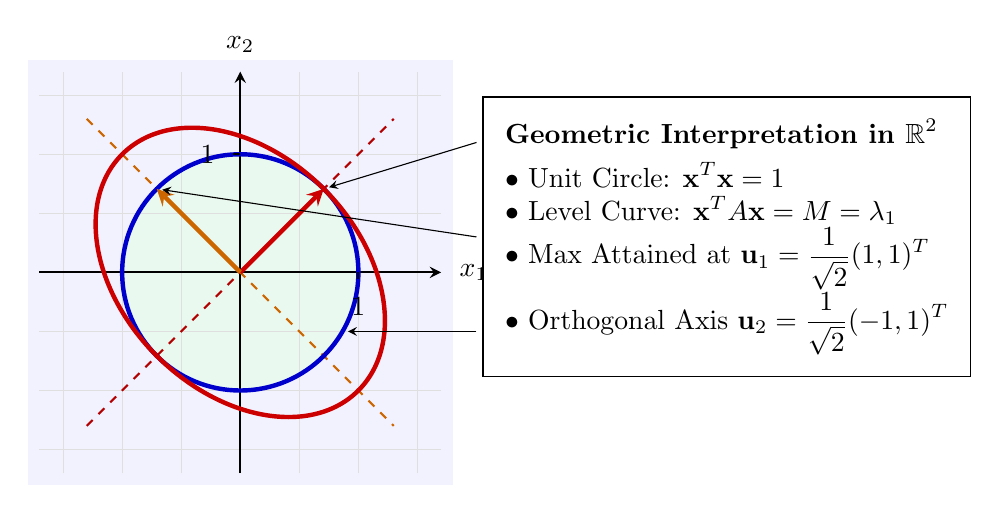
\begin{tikzpicture}[scale=1.5]
    % 1. Background fill
    \fill[blue!5] (-1.8,-1.8) rectangle (1.8,1.8);
    \fill[green!10, opacity=0.6] (0,0) circle (1.0);

    % 2. Grid lines and axes
    \draw[step=0.5, gray!25, thin] (-1.7,-1.7) grid (1.7,1.7);
    \draw[->, >=stealth, thick, black] (-1.7,0) -- (1.7,0) node[right=3pt, black] {$\displaystyle x_1$};
    \draw[->, >=stealth, thick, black] (0,-1.7) -- (0,1.7) node[above=3pt, black] {$\displaystyle x_2$};

    % Principal Axes (u1 and u2)
    \draw[dashed, thick, red!70!black] (-1.3,-1.3) -- (1.3,1.3);
    \draw[dashed, thick, orange!80!black] (-1.3,1.3) -- (1.3,-1.3);

    % 3. Primary plots: Unit circle and level curve ellipse
    \draw[ultra thick, blue!80!black] (0,0) circle (1.0);
    \draw[ultra thick, red!80!black, rotate=45] (0,0) ellipse (1.0 and 1.414);

    % Eigenvector arrows
    \draw[->, >=stealth, ultra thick, red!80!black] (0,0) -- (0.707,0.707);
    \draw[->, >=stealth, ultra thick, orange!80!black] (0,0) -- (-0.707,0.707);

    % Tick marks
    \draw[thick, black] (1.0,0) -- (1.0,-0.06) node[below=3pt, black] {$\displaystyle 1$};
    \draw[thick, black] (0,1.0) -- (-0.06,1.0) node[left=3pt, black] {$\displaystyle 1$};

    % Callout arrows
    \draw[->, >=stealth, shorten >=2pt, thin, black] (2.0, 1.1) -- (0.707, 0.707);
    \draw[->, >=stealth, shorten >=2pt, thin, black] (2.0, 0.3) -- (-0.707, 0.707);
    \draw[->, >=stealth, shorten >=2pt, thin, black] (2.0, -0.5) -- (0.866, -0.5);

    % 4. Labels and Single-Node Legend
    \node[draw=black, fill=white, align=left, inner sep=8pt, anchor=west, text=black] at (2.05, 0.3) {
        \textbf{Geometric Interpretation in $\displaystyle \R^2$}\\[4pt]
        $\displaystyle \bullet\ \text{Unit Circle: } \mathbf{x}^T\mathbf{x} = 1$\\
        $\displaystyle \bullet\ \text{Level Curve: } \mathbf{x}^T A \mathbf{x} = M = \lambda_1$\\
        $\displaystyle \bullet\ \text{Max Attained at } \mathbf{u}_1 = \frac{1}{\sqrt{2}}(1,1)^T$\\
        $\displaystyle \bullet\ \text{Orthogonal Axis } \mathbf{u}_2 = \frac{1}{\sqrt{2}}(-1,1)^T$
    };
\end{tikzpicture}
\end{center}

\subsection{Historical Context and Motivation}
The theory of constrained optimization of quadratic forms emerged in the 18th and 19th centuries through classical mechanics and celestial perturbation theory. Mathematicians such as Leonhard Euler, Joseph-Louis Lagrange, and Augustin-Louis Cauchy sought the principal axes of rigid bodies (the moment of inertia tensor) and the stability of planetary orbits. In 1873, Lord Rayleigh (John William Strutt) introduced the quotient $\mathbf{x}^T A \mathbf{x} / \mathbf{x}^T \mathbf{x}$ in his treatise \emph{The Theory of Sound} to approximate the fundamental resonant frequencies of vibrating continuous elastic systems without solving high-degree polynomial equations directly.

In the early 20th century, Ernst Fischer (1905) and Richard Courant (1920) generalized Rayleigh's variational principle into the celebrated Courant-Fischer Min-Max Theorem (represented in this section by Theorems 6, 7, and 8). In the 1930s, Harold Hotelling realized that sequentially maximizing variance $\mathbf{x}^T \Sigma \mathbf{x}$ subject to unit length $\mathbf{x}^T\mathbf{x} = 1$ and orthogonality $\mathbf{x}^T \mathbf{u}_j = 0$ extracts the most informative uncorrelated features of high-dimensional data—giving birth to Principal Component Analysis (PCA), a cornerstone of modern data science and machine learning.

\subsection{Key Formulas and Theorems}
\begin{theorem}[Theorem 6: Constrained Extrema on the Unit Sphere]
Let $A$ be an $n \times n$ symmetric matrix, and define $m = \min\{\mathbf{x}^T A \mathbf{x} : \|\mathbf{x}\| = 1\}$ and $M = \max\{\mathbf{x}^T A \mathbf{x} : \|\mathbf{x}\| = 1\}$. Then $M$ is the greatest eigenvalue $\lambda_1$ of $A$, and $m$ is the least eigenvalue $\lambda_n$ of $A$. The value of $\mathbf{x}^T A \mathbf{x}$ is $M$ when $\mathbf{x}$ is a unit eigenvector $\mathbf{u}_1$ corresponding to $M$. The value of $\mathbf{x}^T A \mathbf{x}$ is $m$ when $\mathbf{x}$ is a unit eigenvector $\mathbf{u}_n$ corresponding to $m$.
\end{theorem}

\begin{theorem}[Theorem 7: Optimization with One Orthogonality Constraint]
Let $A$, $\lambda_1$, and $\mathbf{u}_1$ be as in Theorem 6. Then the maximum value of $\mathbf{x}^T A \mathbf{x}$ subject to the constraints
\[
\mathbf{x}^T \mathbf{x} = 1, \qquad \mathbf{x}^T \mathbf{u}_1 = 0
\]
is the second greatest eigenvalue, $\lambda_2$, and this maximum is attained when $\mathbf{x}$ is a unit eigenvector $\mathbf{u}_2$ corresponding to $\lambda_2$.
\end{theorem}

\begin{theorem}[Theorem 8: Sequential Variational Characterization of All Eigenvalues]
Let $A$ be a symmetric $n \times n$ matrix with an orthogonal diagonalization $A = P D P^{-1}$, where the entries on the diagonal of $D$ are arranged so that $\lambda_1 \ge \lambda_2 \ge \cdots \ge \lambda_n$ and where the columns of $P$ are corresponding unit eigenvectors $\mathbf{u}_1, \dots, \mathbf{u}_n$. Then for $k = 2, \dots, n$, the maximum value of $\mathbf{x}^T A \mathbf{x}$ subject to the constraints
\[
\mathbf{x}^T \mathbf{x} = 1, \qquad \mathbf{x}^T \mathbf{u}_1 = 0, \quad \dots, \quad \mathbf{x}^T \mathbf{u}_{k-1} = 0
\]
is the eigenvalue $\lambda_k$, and this maximum is attained at $\mathbf{x} = \mathbf{u}_k$.
\end{theorem}

\textbf{Elliptical Constraint Conversion Formula (Example 6 Technique):}
If a quadratic form $q(x, y)$ is constrained by an ellipse $\left(\frac{x}{a}\right)^2 + \left(\frac{y}{b}\right)^2 = 1$ (such as $4x^2 + 9y^2 = 36 \iff (x/3)^2 + (y/2)^2 = 1$), define the normalized coordinates:
\[
x_1 = \frac{x}{a}, \quad x_2 = \frac{y}{b} \quad \Longleftrightarrow \quad x = a x_1, \quad y = b x_2.
\]
Then the constraint becomes $\mathbf{x}^T \mathbf{x} = x_1^2 + x_2^2 = 1$, allowing direct application of Theorem 6 to $Q(\mathbf{x}) = q(ax_1, bx_2)$.

\begin{center}
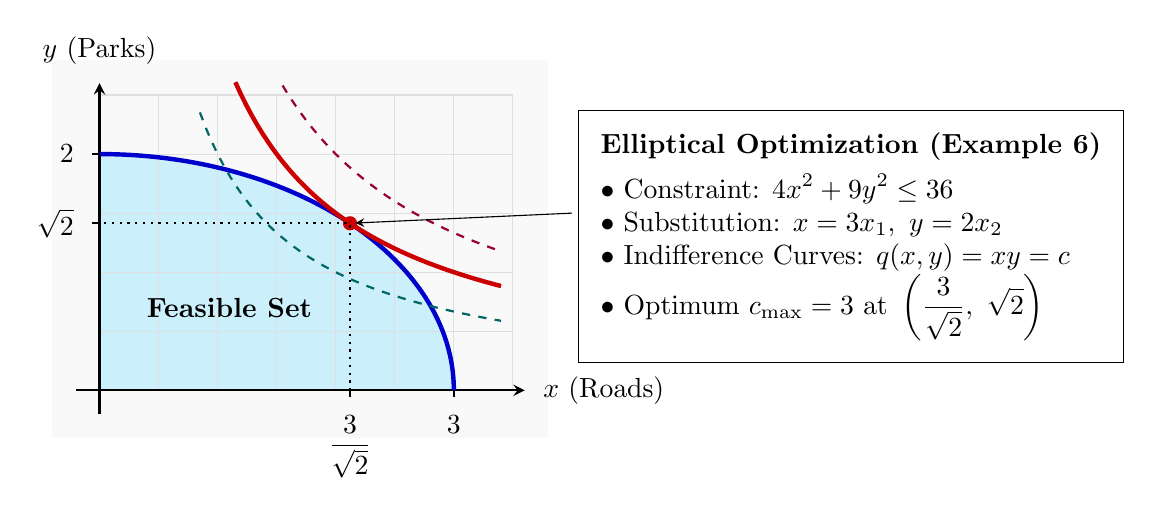
\begin{tikzpicture}[scale=1.5]
    % 1. Background fill
    \fill[gray!5] (-0.4,-0.4) rectangle (3.8,2.8);
    \fill[cyan!20] (0,0) -- (3,0) arc[start angle=0, end angle=90, x radius=3, y radius=2] -- cycle;

    % 2. Grid lines and axes
    \draw[step=0.5, gray!25, thin] (0,0) grid (3.5,2.5);
    \draw[->, >=stealth, thick, black] (-0.2,0) -- (3.6,0) node[right=3pt, black] {$\displaystyle x\text{ (Roads)}$};
    \draw[->, >=stealth, thick, black] (0,-0.2) -- (0,2.6) node[above=3pt, black] {$\displaystyle y\text{ (Parks)}$};

    % 3. Primary plots: Elliptical boundary and indifference curves q(x,y) = xy = c
    \draw[ultra thick, blue!80!black] (3,0) arc[start angle=0, end angle=90, x radius=3, y radius=2];
    \draw[thick, dashed, teal!80!black, domain=0.85:3.4, samples=50] plot (\x, {2.0/\x});
    \draw[ultra thick, red!80!black, domain=1.15:3.4, samples=50] plot (\x, {3.0/\x});
    \draw[thick, dashed, purple!80!black, domain=1.55:3.4, samples=50] plot (\x, {4.0/\x});

    % Optimal tangency point (3/sqrt(2), sqrt(2)) = (2.121, 1.414)
    \fill[red!80!black] (2.121,1.414) circle (0.06);
    \draw[dotted, thick, black] (2.121,0) -- (2.121,1.414) -- (0,1.414);

    % Tick marks
    \draw[thick, black] (3,0) -- (3,-0.06) node[below=3pt, black] {$\displaystyle 3$};
    \draw[thick, black] (2.121,0) -- (2.121,-0.06) node[below=3pt, black] {$\displaystyle \frac{3}{\sqrt{2}}$};
    \draw[thick, black] (0,2) -- (-0.06,2) node[left=3pt, black] {$\displaystyle 2$};
    \draw[thick, black] (0,1.414) -- (-0.06,1.414) node[left=3pt, black] {$\displaystyle \sqrt{2}$};

    % Callout arrow
    \draw[->, >=stealth, shorten >=2pt, thin, black] (4.0, 1.5) -- (2.121, 1.414);

    % 4. Labels and Single-Node Legend
    \node[text=black] at (1.1, 0.7) {\textbf{Feasible Set}};
    \node[draw=black, fill=white, align=left, inner sep=8pt, anchor=west, text=black] at (4.05, 1.3) {
        \textbf{Elliptical Optimization (Example 6)}\\[4pt]
        $\displaystyle \bullet\ \text{Constraint: } 4x^2 + 9y^2 \le 36$\\
        $\displaystyle \bullet\ \text{Substitution: } x = 3x_1,\ y = 2x_2$\\
        $\displaystyle \bullet\ \text{Indifference Curves: } q(x,y) = xy = c$\\
        $\displaystyle \bullet\ \text{Optimum } c_{\max} = 3 \text{ at } \left(\frac{3}{\sqrt{2}},\ \sqrt{2}\right)$
    };
\end{tikzpicture}
\end{center}

\subsection{Prerequisites}
To master Section 7.3, you must have complete fluency in the following foundational topics:
\begin{itemize}
    \item \textbf{Matrix of a Quadratic Form (Section 7.2):} Converting $Q(\mathbf{x}) = \sum_{i=1}^n a_{ii} x_i^2 + \sum_{i < j} c_{ij} x_i x_j$ into $\mathbf{x}^T A \mathbf{x}$ by setting $a_{ii}$ on the diagonal and splitting each cross-product coefficient equally: $a_{ij} = a_{ji} = \frac{1}{2} c_{ij}$.
    \item \textbf{Eigenvalues and Eigenvectors (Chapter 5):} Solving $\det(A - \lambda I) = 0$ and finding bases for $\operatorname{Nul}(A - \lambda I)$ via Gaussian row reduction.
    \item \textbf{Orthogonality and Normalization (Chapter 6):} Computing Euclidean norms $\|\mathbf{v}\| = \sqrt{\mathbf{v}^T \mathbf{v}}$, normalizing $\mathbf{u} = \mathbf{v}/\|\mathbf{v}\|$, and applying the Gram-Schmidt process when an eigenvalue has geometric multiplicity greater than $1$.
    \item \textbf{Orthogonal Diagonalization of Symmetric Matrices (Section 7.1):} Constructing an orthogonal matrix $P$ ($P^T P = I$) such that $A = P D P^T$, and knowing that eigenvectors corresponding to distinct eigenvalues of a symmetric matrix are automatically orthogonal.
\end{itemize}

\newpage
% ============================================================================
% PART 2: DETAILED HOMEWORK SOLUTIONS
% ============================================================================
\section{Detailed Homework Solutions}

\subsection{Practice Problems}

\textbf{Practice Problem 1.} \emph{Let $Q(\mathbf{x}) = 3x_1^2 + 3x_2^2 + 2x_1x_2$. Find a change of variable that transforms $Q$ into a quadratic form with no cross-product term, and give the new quadratic form.}

\textbf{Solution:}
\begin{enumerate}[label=\textbf{Step \arabic*:}]
    \item \textbf{Construct the Symmetric Matrix $A$:}
    The squared terms have coefficients $a_{11} = 3$ and $a_{22} = 3$. The cross-product term $2x_1x_2$ has coefficient $2$, so we place half of it ($2/2 = 1$) in the $(1,2)$ and $(2,1)$ entries:
    \[
    A = \begin{bmatrix} 3 & 1 \\ 1 & 3 \end{bmatrix}.
    \]
    \item \textbf{Find the Eigenvalues of $A$:}
    Compute the characteristic polynomial $\det(A - \lambda I) = 0$:
    \[
    \det \begin{bmatrix} 3 - \lambda & 1 \\ 1 & 3 - \lambda \end{bmatrix} = (3 - \lambda)^2 - 1 = \lambda^2 - 6\lambda + 8 = (\lambda - 4)(\lambda - 2) = 0.
    \]
    Ordered from greatest to least, the eigenvalues are $\lambda_1 = 4$ and $\lambda_2 = 2$.
    \item \textbf{Find Corresponding Orthonormal Eigenvectors:}
    \begin{itemize}
        \item For $\lambda_1 = 4$: Solve $(A - 4I)\mathbf{x} = \mathbf{0}$:
        \[
        \begin{bmatrix} -1 & 1 \\ 1 & -1 \end{bmatrix} \begin{bmatrix} x_1 \\ x_2 \end{bmatrix} = \begin{bmatrix} 0 \\ 0 \end{bmatrix} \implies -x_1 + x_2 = 0 \implies x_1 = x_2.
        \]
        Choosing $x_2 = 1$ gives $\mathbf{v}_1 = \begin{bmatrix} 1 \\ 1 \end{bmatrix}$ with norm $\|\mathbf{v}_1\| = \sqrt{1^2 + 1^2} = \sqrt{2}$. Normalizing yields:
        \[
        \mathbf{u}_1 = \frac{\mathbf{v}_1}{\|\mathbf{v}_1\|} = \begin{bmatrix} 1/\sqrt{2} \\ 1/\sqrt{2} \end{bmatrix}.
        \]
        \item For $\lambda_2 = 2$: Solve $(A - 2I)\mathbf{x} = \mathbf{0}$:
        \[
        \begin{bmatrix} 1 & 1 \\ 1 & 1 \end{bmatrix} \begin{bmatrix} x_1 \\ x_2 \end{bmatrix} = \begin{bmatrix} 0 \\ 0 \end{bmatrix} \implies x_1 + x_2 = 0 \implies x_1 = -x_2.
        \]
        Choosing $x_2 = 1$ gives $\mathbf{v}_2 = \begin{bmatrix} -1 \\ 1 \end{bmatrix}$ with norm $\|\mathbf{v}_2\| = \sqrt{(-1)^2 + 1^2} = \sqrt{2}$. Normalizing yields:
        \[
        \mathbf{u}_2 = \frac{\mathbf{v}_2}{\|\mathbf{v}_2\|} = \begin{bmatrix} -1/\sqrt{2} \\ 1/\sqrt{2} \end{bmatrix}.
        \]
    \end{itemize}
    \item \textbf{Form the Orthogonal Change of Variable and New Quadratic Form:}
    Assemble $P = \begin{bmatrix} \mathbf{u}_1 & \mathbf{u}_2 \end{bmatrix}$ and $D = \operatorname{diag}(4, 2)$:
    \[
    P = \begin{bmatrix} 1/\sqrt{2} & -1/\sqrt{2} \\ 1/\sqrt{2} & 1/\sqrt{2} \end{bmatrix}, \qquad \mathbf{x} = P\mathbf{y}.
    \]
    Under $\mathbf{x} = P\mathbf{y}$, the quadratic form transforms into:
    \[
    Q(P\mathbf{y}) = \mathbf{y}^T D \mathbf{y} = 4y_1^2 + 2y_2^2.
    \]
\end{enumerate}
\textbf{Final Answer:} The change of variable is $\mathbf{x} = P\mathbf{y}$ with $P = \begin{bmatrix} 1/\sqrt{2} & -1/\sqrt{2} \\ 1/\sqrt{2} & 1/\sqrt{2} \end{bmatrix}$, and the new quadratic form is $4y_1^2 + 2y_2^2$.

\medskip
\hrule
\medskip

\textbf{Practice Problem 2.} \emph{With $Q$ as in Problem 1, find the maximum value of $Q(\mathbf{x})$ subject to the constraint $\mathbf{x}^T\mathbf{x} = 1$, and find a unit vector at which the maximum is attained.}

\textbf{Solution:}
\begin{enumerate}[label=\textbf{Step \arabic*:}]
    \item \textbf{Identify the Maximum Value via Theorem 6:}
    By Theorem 6, the maximum value of $Q(\mathbf{x}) = \mathbf{x}^T A \mathbf{x}$ subject to $\mathbf{x}^T\mathbf{x} = 1$ is the greatest eigenvalue $\lambda_1$ of $A$. From Practice Problem 1, the eigenvalues of $A$ are $4$ and $2$, so the maximum value is $\lambda_1 = 4$.
    \item \textbf{Identify the Maximizing Unit Vector:}
    By Theorem 6, the maximum value $\lambda_1 = 4$ is attained at the corresponding unit eigenvector $\mathbf{u}_1$ of $A$ (not $\mathbf{e}_1 = (1,0)^T$, which maximizes $\mathbf{y}^T D \mathbf{y}$ in $\mathbf{y}$-coordinates):
    \[
    \mathbf{u}_1 = \begin{bmatrix} 1/\sqrt{2} \\ 1/\sqrt{2} \end{bmatrix} \quad \left(\text{or } -\mathbf{u}_1 = \begin{bmatrix} -1/\sqrt{2} \\ -1/\sqrt{2} \end{bmatrix}\right).
    \]
\end{enumerate}
\textbf{Final Answer:} The maximum value of $Q(\mathbf{x})$ subject to $\mathbf{x}^T\mathbf{x} = 1$ is $4$, attained at the unit vector $\mathbf{u}_1 = \begin{bmatrix} 1/\sqrt{2} \\ 1/\sqrt{2} \end{bmatrix}$.

\newpage
\subsection{Section 7.3 Exercises}

\textbf{Exercise 1.} \emph{Find the change of variable $\mathbf{x} = P\mathbf{y}$ that transforms the quadratic form $\mathbf{x}^T A \mathbf{x}$ into $\mathbf{y}^T D \mathbf{y}$ as shown:}
\[
5x_1^2 + 4x_2^2 + 3x_3^2 + 4x_1x_2 + 4x_2x_3 = 7y_1^2 + 4y_2^2 + y_3^2.
\]

\textbf{Solution:}
\begin{enumerate}[label=\textbf{Step \arabic*:}]
    \item \textbf{Construct Matrices $A$ and $D$:}
    The symmetric matrix $A$ of the left-hand quadratic form and the diagonal matrix $D$ of the right-hand quadratic form are:
    \[
    A = \begin{bmatrix} 5 & 2 & 0 \\ 2 & 4 & 2 \\ 0 & 2 & 3 \end{bmatrix}, \qquad D = \begin{bmatrix} 7 & 0 & 0 \\ 0 & 4 & 0 \\ 0 & 0 & 1 \end{bmatrix}.
    \]
    Since $A = P D P^T$, the diagonal entries of $D$ are precisely the eigenvalues of $A$: $\lambda_1 = 7$, $\lambda_2 = 4$, and $\lambda_3 = 1$.
    \item \textbf{Find Unit Eigenvector $\mathbf{u}_1$ for $\lambda_1 = 7$:}
    Row reduce $A - 7I$:
    \[
    A - 7I = \begin{bmatrix} -2 & 2 & 0 \\ 2 & -3 & 2 \\ 0 & 2 & -4 \end{bmatrix} \sim \begin{bmatrix} 1 & -1 & 0 \\ 0 & -1 & 2 \\ 0 & 2 & -4 \end{bmatrix} \sim \begin{bmatrix} 1 & 0 & -2 \\ 0 & 1 & -2 \\ 0 & 0 & 0 \end{bmatrix}.
    \]
    Thus $x_1 = 2x_3$ and $x_2 = 2x_3$. Setting $x_3 = 1$ gives $\mathbf{v}_1 = \begin{bmatrix} 2 \\ 2 \\ 1 \end{bmatrix}$ with norm $\|\mathbf{v}_1\| = \sqrt{2^2 + 2^2 + 1^2} = \sqrt{9} = 3$. Normalizing yields:
    \[
    \mathbf{u}_1 = \begin{bmatrix} 2/3 \\ 2/3 \\ 1/3 \end{bmatrix}.
    \]
    \item \textbf{Find Unit Eigenvector $\mathbf{u}_2$ for $\lambda_2 = 4$:}
    Row reduce $A - 4I$:
    \[
    A - 4I = \begin{bmatrix} 1 & 2 & 0 \\ 2 & 0 & 2 \\ 0 & 2 & -1 \end{bmatrix} \sim \begin{bmatrix} 1 & 2 & 0 \\ 0 & -4 & 2 \\ 0 & 2 & -1 \end{bmatrix} \sim \begin{bmatrix} 1 & 0 & 1 \\ 0 & 1 & -1/2 \\ 0 & 0 & 0 \end{bmatrix}.
    \]
    Thus $x_1 = -x_3$ and $x_2 = \frac{1}{2}x_3$. Setting $x_3 = 2$ gives $\mathbf{v}_2 = \begin{bmatrix} -2 \\ 1 \\ 2 \end{bmatrix}$ with norm $\|\mathbf{v}_2\| = \sqrt{(-2)^2 + 1^2 + 2^2} = 3$. Normalizing yields:
    \[
    \mathbf{u}_2 = \begin{bmatrix} -2/3 \\ 1/3 \\ 2/3 \end{bmatrix}.
    \]
    \item \textbf{Find Unit Eigenvector $\mathbf{u}_3$ for $\lambda_3 = 1$:}
    Row reduce $A - I$:
    \[
    A - I = \begin{bmatrix} 4 & 2 & 0 \\ 2 & 3 & 2 \\ 0 & 2 & 2 \end{bmatrix} \sim \begin{bmatrix} 2 & 1 & 0 \\ 0 & 2 & 2 \\ 0 & 2 & 2 \end{bmatrix} \sim \begin{bmatrix} 1 & 1/2 & 0 \\ 0 & 1 & 1 \\ 0 & 0 & 0 \end{bmatrix} \sim \begin{bmatrix} 1 & 0 & -1/2 \\ 0 & 1 & 1 \\ 0 & 0 & 0 \end{bmatrix}.
    \]
    Thus $x_1 = \frac{1}{2}x_3$ and $x_2 = -x_3$. Setting $x_3 = 2$ gives $\mathbf{v}_3 = \begin{bmatrix} 1 \\ -2 \\ 2 \end{bmatrix}$ with norm $\|\mathbf{v}_3\| = \sqrt{1^2 + (-2)^2 + 2^2} = 3$. Normalizing yields:
    \[
    \mathbf{u}_3 = \begin{bmatrix} 1/3 \\ -2/3 \\ 2/3 \end{bmatrix}.
    \]
\end{enumerate}
\textbf{Final Answer:} The change of variable is $\mathbf{x} = P\mathbf{y}$, where
\[
P = \begin{bmatrix} \mathbf{u}_1 & \mathbf{u}_2 & \mathbf{u}_3 \end{bmatrix} = \begin{bmatrix} 2/3 & -2/3 & 1/3 \\ 2/3 & 1/3 & -2/3 \\ 1/3 & 2/3 & 2/3 \end{bmatrix} = \frac{1}{3} \begin{bmatrix} 2 & -2 & 1 \\ 2 & 1 & -2 \\ 1 & 2 & 2 \end{bmatrix}
\]
(where any column of $P$ may be multiplied by $-1$).

\medskip
\hrule
\medskip

\textbf{Exercise 2.} \emph{Find the change of variable $\mathbf{x} = P\mathbf{y}$ that transforms the quadratic form $\mathbf{x}^T A \mathbf{x}$ into $\mathbf{y}^T D \mathbf{y}$ as shown:}
\[
5x_1^2 + 5x_2^2 + 3x_3^2 + 10x_1x_2 + 4x_1x_3 + 4x_2x_3 = 11y_1^2 + 2y_2^2.
\]
\emph{Hint: $\mathbf{x}$ and $\mathbf{y}$ must have the same number of coordinates, so the quadratic form shown here must have a coefficient of zero for $y_3^2$.}

\textbf{Solution:}
\begin{enumerate}[label=\textbf{Step \arabic*:}]
    \item \textbf{Construct Matrices $A$ and $D$:}
    The right-hand quadratic form is $11y_1^2 + 2y_2^2 + 0y_3^2$, so the matrices $A$ and $D$ are:
    \[
    A = \begin{bmatrix} 5 & 5 & 2 \\ 5 & 5 & 2 \\ 2 & 2 & 3 \end{bmatrix}, \qquad D = \begin{bmatrix} 11 & 0 & 0 \\ 0 & 2 & 0 \\ 0 & 0 & 0 \end{bmatrix}.
    \]
    The eigenvalues of $A$ are $\lambda_1 = 11$, $\lambda_2 = 2$, and $\lambda_3 = 0$.
    \item \textbf{Find Unit Eigenvector $\mathbf{u}_1$ for $\lambda_1 = 11$:}
    Row reduce $A - 11I$:
    \[
    A - 11I = \begin{bmatrix} -6 & 5 & 2 \\ 5 & -6 & 2 \\ 2 & 2 & -8 \end{bmatrix} \sim \begin{bmatrix} -11 & 11 & 0 \\ 5 & -6 & 2 \\ 1 & 1 & -4 \end{bmatrix} \sim \begin{bmatrix} 1 & -1 & 0 \\ 0 & -1 & 2 \\ 0 & 2 & -4 \end{bmatrix} \sim \begin{bmatrix} 1 & 0 & -2 \\ 0 & 1 & -2 \\ 0 & 0 & 0 \end{bmatrix}.
    \]
    Thus $x_1 = 2x_3$ and $x_2 = 2x_3$. Setting $x_3 = 1$ gives $\mathbf{v}_1 = \begin{bmatrix} 2 \\ 2 \\ 1 \end{bmatrix}$ with norm $\|\mathbf{v}_1\| = \sqrt{4 + 4 + 1} = 3$. Normalizing yields:
    \[
    \mathbf{u}_1 = \begin{bmatrix} 2/3 \\ 2/3 \\ 1/3 \end{bmatrix}.
    \]
    \item \textbf{Find Unit Eigenvector $\mathbf{u}_2$ for $\lambda_2 = 2$:}
    Row reduce $A - 2I$:
    \[
    A - 2I = \begin{bmatrix} 3 & 5 & 2 \\ 5 & 3 & 2 \\ 2 & 2 & 1 \end{bmatrix} \sim \begin{bmatrix} -2 & 2 & 0 \\ 5 & 3 & 2 \\ 2 & 2 & 1 \end{bmatrix} \sim \begin{bmatrix} 1 & -1 & 0 \\ 0 & 8 & 2 \\ 0 & 4 & 1 \end{bmatrix} \sim \begin{bmatrix} 1 & 0 & 1/4 \\ 0 & 1 & 1/4 \\ 0 & 0 & 0 \end{bmatrix}.
    \]
    Thus $x_1 = -\frac{1}{4}x_3$ and $x_2 = -\frac{1}{4}x_3$. Setting $x_3 = -4$ gives $\mathbf{v}_2 = \begin{bmatrix} 1 \\ 1 \\ -4 \end{bmatrix}$ with norm $\|\mathbf{v}_2\| = \sqrt{1^2 + 1^2 + (-4)^2} = \sqrt{18} = 3\sqrt{2}$. Normalizing yields:
    \[
    \mathbf{u}_2 = \begin{bmatrix} 1/(3\sqrt{2}) \\ 1/(3\sqrt{2}) \\ -4/(3\sqrt{2}) \end{bmatrix}.
    \]
    \item \textbf{Find Unit Eigenvector $\mathbf{u}_3$ for $\lambda_3 = 0$:}
    Row reduce $A - 0I = A$:
    \[
    A = \begin{bmatrix} 5 & 5 & 2 \\ 5 & 5 & 2 \\ 2 & 2 & 3 \end{bmatrix} \sim \begin{bmatrix} 1 & 1 & 0 \\ 0 & 0 & 1 \\ 0 & 0 & 0 \end{bmatrix}.
    \]
    Thus $x_1 = -x_2$ and $x_3 = 0$. Setting $x_2 = 1$ gives $\mathbf{v}_3 = \begin{bmatrix} -1 \\ 1 \\ 0 \end{bmatrix}$ with norm $\|\mathbf{v}_3\| = \sqrt{(-1)^2 + 1^2 + 0^2} = \sqrt{2}$. Normalizing yields:
    \[
    \mathbf{u}_3 = \begin{bmatrix} -1/\sqrt{2} \\ 1/\sqrt{2} \\ 0 \end{bmatrix}.
    \]
\end{enumerate}
\textbf{Final Answer:} The change of variable is $\mathbf{x} = P\mathbf{y}$, where
\[
P = \begin{bmatrix} \mathbf{u}_1 & \mathbf{u}_2 & \mathbf{u}_3 \end{bmatrix} = \begin{bmatrix} 2/3 & 1/(3\sqrt{2}) & -1/\sqrt{2} \\ 2/3 & 1/(3\sqrt{2}) & 1/\sqrt{2} \\ 1/3 & -4/(3\sqrt{2}) & 0 \end{bmatrix}.
\]

\medskip
\hrule
\medskip

\textbf{Exercise 3.} \emph{For $Q(\mathbf{x}) = 5x_1^2 + 4x_2^2 + 3x_3^2 + 4x_1x_2 + 4x_2x_3$ (see Exercise 1), find (a) the maximum value of $Q(\mathbf{x})$ subject to the constraint $\mathbf{x}^T\mathbf{x} = 1$, (b) a unit vector $\mathbf{u}$ where this maximum is attained, and (c) the maximum of $Q(\mathbf{x})$ subject to the constraints $\mathbf{x}^T\mathbf{x} = 1$ and $\mathbf{x}^T\mathbf{u} = 0$.}

\textbf{Solution:}
From Exercise 1, the orthogonally diagonalized form of $Q(\mathbf{x})$ is $\mathbf{y}^T D \mathbf{y} = 7y_1^2 + 4y_2^2 + y_3^2$, so the eigenvalues of $A$ ordered from greatest to least are $\lambda_1 = 7$, $\lambda_2 = 4$, and $\lambda_3 = 1$.
\begin{enumerate}[label=(\alph*)]
    \item By Theorem 6, the maximum value of $Q(\mathbf{x})$ subject to $\mathbf{x}^T\mathbf{x} = 1$ is the greatest eigenvalue of $A$:
    \[
    M = \lambda_1 = 7.
    \]
    \item By Theorem 6, this maximum is attained at a unit eigenvector $\mathbf{u}$ corresponding to $\lambda_1 = 7$. From Exercise 1, Step 2:
    \[
    \mathbf{u} = \mathbf{u}_1 = \begin{bmatrix} 2/3 \\ 2/3 \\ 1/3 \end{bmatrix} \quad \left(\text{or } \begin{bmatrix} -2/3 \\ -2/3 \\ -1/3 \end{bmatrix}\right).
    \]
    \item By Theorem 7, the maximum value of $Q(\mathbf{x})$ subject to $\mathbf{x}^T\mathbf{x} = 1$ and $\mathbf{x}^T\mathbf{u} = 0$ is the second greatest eigenvalue of $A$:
    \[
    \lambda_2 = 4.
    \]
\end{enumerate}
\textbf{Final Answer:} (a) $7$; \quad (b) $\mathbf{u} = \begin{bmatrix} 2/3 \\ 2/3 \\ 1/3 \end{bmatrix}$; \quad (c) $4$.

\medskip
\hrule
\medskip

\textbf{Exercise 4.} \emph{For $Q(\mathbf{x}) = 5x_1^2 + 5x_2^2 + 3x_3^2 + 10x_1x_2 + 4x_1x_3 + 4x_2x_3$ (see Exercise 2), find (a) the maximum value of $Q(\mathbf{x})$ subject to the constraint $\mathbf{x}^T\mathbf{x} = 1$, (b) a unit vector $\mathbf{u}$ where this maximum is attained, and (c) the maximum of $Q(\mathbf{x})$ subject to the constraints $\mathbf{x}^T\mathbf{x} = 1$ and $\mathbf{x}^T\mathbf{u} = 0$.}

\textbf{Solution:}
From Exercise 2, the orthogonally diagonalized form of $Q(\mathbf{x})$ is $\mathbf{y}^T D \mathbf{y} = 11y_1^2 + 2y_2^2 + 0y_3^2$, so the eigenvalues of $A$ ordered from greatest to least are $\lambda_1 = 11$, $\lambda_2 = 2$, and $\lambda_3 = 0$.
\begin{enumerate}[label=(\alph*)]
    \item By Theorem 6, the maximum value of $Q(\mathbf{x})$ subject to $\mathbf{x}^T\mathbf{x} = 1$ is the greatest eigenvalue of $A$:
    \[
    M = \lambda_1 = 11.
    \]
    \item By Theorem 6, this maximum is attained at a unit eigenvector $\mathbf{u}$ corresponding to $\lambda_1 = 11$. From Exercise 2, Step 2:
    \[
    \mathbf{u} = \mathbf{u}_1 = \begin{bmatrix} 2/3 \\ 2/3 \\ 1/3 \end{bmatrix} \quad \left(\text{or } \begin{bmatrix} -2/3 \\ -2/3 \\ -1/3 \end{bmatrix}\right).
    \]
    \item By Theorem 7, the maximum value of $Q(\mathbf{x})$ subject to $\mathbf{x}^T\mathbf{x} = 1$ and $\mathbf{x}^T\mathbf{u} = 0$ is the second greatest eigenvalue of $A$:
    \[
    \lambda_2 = 2.
    \]
\end{enumerate}
\textbf{Final Answer:} (a) $11$; \quad (b) $\mathbf{u} = \begin{bmatrix} 2/3 \\ 2/3 \\ 1/3 \end{bmatrix}$; \quad (c) $2$.

\medskip
\hrule
\medskip

\textbf{Exercise 5.} \emph{For $Q(\mathbf{x}) = x_1^2 + x_2^2 - 12x_1x_2$, find (a) the maximum value of $Q(\mathbf{x})$ subject to the constraint $\mathbf{x}^T\mathbf{x} = 1$, (b) a unit vector $\mathbf{u}$ where this maximum is attained, and (c) the maximum of $Q(\mathbf{x})$ subject to the constraints $\mathbf{x}^T\mathbf{x} = 1$ and $\mathbf{x}^T\mathbf{u} = 0$.}

\textbf{Solution:}
\begin{enumerate}[label=\textbf{Step \arabic*:}]
    \item \textbf{Construct Matrix $A$ and Find Eigenvalues:}
    The symmetric matrix of $Q(\mathbf{x}) = x_1^2 + x_2^2 - 12x_1x_2$ is:
    \[
    A = \begin{bmatrix} 1 & -6 \\ -6 & 1 \end{bmatrix}.
    \]
    Solve the characteristic equation $\det(A - \lambda I) = 0$:
    \[
    (1 - \lambda)^2 - (-6)^2 = \lambda^2 - 2\lambda + 1 - 36 = \lambda^2 - 2\lambda - 35 = (\lambda - 7)(\lambda + 5) = 0.
    \]
    Thus the eigenvalues are $\lambda_1 = 7$ and $\lambda_2 = -5$.
    \item \textbf{Answer Part (a):}
    By Theorem 6, the maximum value of $Q(\mathbf{x})$ subject to $\mathbf{x}^T\mathbf{x} = 1$ is $\lambda_1 = 7$.
    \item \textbf{Answer Part (b):}
    Find a unit eigenvector for $\lambda_1 = 7$ by solving $(A - 7I)\mathbf{x} = \mathbf{0}$:
    \[
    \begin{bmatrix} -6 & -6 \\ -6 & -6 \end{bmatrix} \begin{bmatrix} x_1 \\ x_2 \end{bmatrix} = \begin{bmatrix} 0 \\ 0 \end{bmatrix} \implies x_1 + x_2 = 0 \implies x_1 = -x_2.
    \]
    Setting $x_2 = 1$ gives $\mathbf{v}_1 = \begin{bmatrix} -1 \\ 1 \end{bmatrix}$ (or $\begin{bmatrix} 1 \\ -1 \end{bmatrix}$) with norm $\|\mathbf{v}_1\| = \sqrt{(-1)^2 + 1^2} = \sqrt{2}$. Normalizing yields:
    \[
    \mathbf{u} = \begin{bmatrix} -1/\sqrt{2} \\ 1/\sqrt{2} \end{bmatrix} \quad \left(\text{or } \begin{bmatrix} 1/\sqrt{2} \\ -1/\sqrt{2} \end{bmatrix}\right).
    \]
    \item \textbf{Answer Part (c):}
    By Theorem 7, the maximum value of $Q(\mathbf{x})$ subject to $\mathbf{x}^T\mathbf{x} = 1$ and $\mathbf{x}^T\mathbf{u} = 0$ is the second greatest eigenvalue, $\lambda_2 = -5$.
\end{enumerate}
\textbf{Final Answer:} (a) $7$; \quad (b) $\mathbf{u} = \begin{bmatrix} -1/\sqrt{2} \\ 1/\sqrt{2} \end{bmatrix}$ (or $\begin{bmatrix} 1/\sqrt{2} \\ -1/\sqrt{2} \end{bmatrix}$); \quad (c) $-5$.

\medskip
\hrule
\medskip

\textbf{Exercise 6.} \emph{For $Q(\mathbf{x}) = 4x_1^2 + 7x_2^2 + 4x_1x_2$, find (a) the maximum value of $Q(\mathbf{x})$ subject to the constraint $\mathbf{x}^T\mathbf{x} = 1$, (b) a unit vector $\mathbf{u}$ where this maximum is attained, and (c) the maximum of $Q(\mathbf{x})$ subject to the constraints $\mathbf{x}^T\mathbf{x} = 1$ and $\mathbf{x}^T\mathbf{u} = 0$.}

\textbf{Solution:}
\begin{enumerate}[label=\textbf{Step \arabic*:}]
    \item \textbf{Construct Matrix $A$ and Find Eigenvalues:}
    The symmetric matrix of $Q(\mathbf{x}) = 4x_1^2 + 7x_2^2 + 4x_1x_2$ is:
    \[
    A = \begin{bmatrix} 4 & 2 \\ 2 & 7 \end{bmatrix}.
    \]
    Solve the characteristic equation $\det(A - \lambda I) = 0$:
    \[
    (4 - \lambda)(7 - \lambda) - 4 = \lambda^2 - 11\lambda + 28 - 4 = \lambda^2 - 11\lambda + 24 = (\lambda - 8)(\lambda - 3) = 0.
    \]
    Thus the eigenvalues are $\lambda_1 = 8$ and $\lambda_2 = 3$.
    \item \textbf{Answer Part (a):}
    By Theorem 6, the maximum value of $Q(\mathbf{x})$ subject to $\mathbf{x}^T\mathbf{x} = 1$ is $\lambda_1 = 8$.
    \item \textbf{Answer Part (b):}
    Find a unit eigenvector for $\lambda_1 = 8$ by solving $(A - 8I)\mathbf{x} = \mathbf{0}$:
    \[
    \begin{bmatrix} -4 & 2 \\ 2 & -1 \end{bmatrix} \begin{bmatrix} x_1 \\ x_2 \end{bmatrix} = \begin{bmatrix} 0 \\ 0 \end{bmatrix} \implies 2x_1 - x_2 = 0 \implies x_2 = 2x_1.
    \]
    Setting $x_1 = 1$ gives $\mathbf{v}_1 = \begin{bmatrix} 1 \\ 2 \end{bmatrix}$ with norm $\|\mathbf{v}_1\| = \sqrt{1^2 + 2^2} = \sqrt{5}$. Normalizing yields:
    \[
    \mathbf{u} = \begin{bmatrix} 1/\sqrt{5} \\ 2/\sqrt{5} \end{bmatrix} \quad \left(\text{or } \begin{bmatrix} -1/\sqrt{5} \\ -2/\sqrt{5} \end{bmatrix}\right).
    \]
    \item \textbf{Answer Part (c):}
    By Theorem 7, the maximum value of $Q(\mathbf{x})$ subject to $\mathbf{x}^T\mathbf{x} = 1$ and $\mathbf{x}^T\mathbf{u} = 0$ is the second greatest eigenvalue, $\lambda_2 = 3$.
\end{enumerate}
\textbf{Final Answer:} (a) $8$; \quad (b) $\mathbf{u} = \begin{bmatrix} 1/\sqrt{5} \\ 2/\sqrt{5} \end{bmatrix}$; \quad (c) $3$.

\medskip
\hrule
\medskip

\textbf{Exercise 7.} \emph{Let $Q(\mathbf{x}) = -3x_1^2 - 4x_2^2 + 4x_1x_2 - 4x_2x_3$. Find a unit vector $\mathbf{x}$ in $\mathbb{R}^3$ at which $Q(\mathbf{x})$ is maximized, subject to $\mathbf{x}^T\mathbf{x} = 1$. [Hint: The eigenvalues of the matrix of the quadratic form $Q$ are $1, -2$, and $-6$.]}

\textbf{Solution:}
\begin{enumerate}[label=\textbf{Step \arabic*:}]
    \item \textbf{Construct Matrix $A$ and Identify Greatest Eigenvalue:}
    Note that the $x_3^2$ and $x_1x_3$ coefficients are $0$. The symmetric matrix $A$ is:
    \[
    A = \begin{bmatrix} -3 & 2 & 0 \\ 2 & -4 & -2 \\ 0 & -2 & 0 \end{bmatrix}.
    \]
    In the standard ordering of real numbers, $-6 < -2 < 1$, so the greatest eigenvalue is $\lambda_1 = 1$.
    \item \textbf{Find a Unit Eigenvector for $\lambda_1 = 1$:}
    Row reduce $A - 1I$:
    \[
    A - I = \begin{bmatrix} -4 & 2 & 0 \\ 2 & -5 & -2 \\ 0 & -2 & -1 \end{bmatrix} \sim \begin{bmatrix} 2 & -1 & 0 \\ 0 & -4 & -2 \\ 0 & -2 & -1 \end{bmatrix} \sim \begin{bmatrix} 1 & 0 & 1/4 \\ 0 & 1 & 1/2 \\ 0 & 0 & 0 \end{bmatrix}.
    \]
    Thus $x_1 = -\frac{1}{4}x_3$ and $x_2 = -\frac{1}{2}x_3$. Setting $x_3 = -4$ gives $\mathbf{v}_1 = \begin{bmatrix} 1 \\ 2 \\ -4 \end{bmatrix}$.
    Compute the Euclidean length of $\mathbf{v}_1$:
    \[
    \|\mathbf{v}_1\| = \sqrt{1^2 + 2^2 + (-4)^2} = \sqrt{1 + 4 + 16} = \sqrt{21}.
    \]
    Normalizing $\mathbf{v}_1$ yields the maximizing unit vector $\mathbf{x}$.
\end{enumerate}
\textbf{Final Answer:} $\mathbf{x} = \begin{bmatrix} 1/\sqrt{21} \\ 2/\sqrt{21} \\ -4/\sqrt{21} \end{bmatrix}$ (or $\begin{bmatrix} -1/\sqrt{21} \\ -2/\sqrt{21} \\ 4/\sqrt{21} \end{bmatrix}$).

\medskip
\hrule
\medskip

\textbf{Exercise 8.} \emph{Let $Q(\mathbf{x}) = 4x_1^2 + 7x_2^2 + 4x_3^2 - 4x_1x_2 + 8x_1x_3 + 4x_2x_3$. Find a unit vector $\mathbf{x}$ in $\mathbb{R}^3$ at which $Q(\mathbf{x})$ is maximized, subject to $\mathbf{x}^T\mathbf{x} = 1$. [Hint: The eigenvalues of the matrix of the quadratic form $Q$ are $8$ and $-1$.]}

\textbf{Solution:}
\begin{enumerate}[label=\textbf{Step \arabic*:}]
    \item \textbf{Construct Matrix $A$ and Identify Greatest Eigenvalue:}
    The symmetric matrix $A$ of the quadratic form is:
    \[
    A = \begin{bmatrix} 4 & -2 & 4 \\ -2 & 7 & 2 \\ 4 & 2 & 4 \end{bmatrix}.
    \]
    The greatest eigenvalue is $\lambda_1 = 8$ (which has multiplicity $2$, since $\operatorname{tr}(A) = 4 + 7 + 4 = 15 = 8 + 8 + (-1)$).
    \item \textbf{Find the Eigenspace for $\lambda_1 = 8$:}
    Row reduce $A - 8I$:
    \[
    A - 8I = \begin{bmatrix} -4 & -2 & 4 \\ -2 & -1 & 2 \\ 4 & 2 & -4 \end{bmatrix} \sim \begin{bmatrix} 2 & 1 & -2 \\ 0 & 0 & 0 \\ 0 & 0 & 0 \end{bmatrix}.
    \]
    Every nonzero vector satisfying $2x_1 + x_2 - 2x_3 = 0 \iff x_2 = -2x_1 + 2x_3$ is an eigenvector for $\lambda_1 = 8$:
    \[
    \mathbf{v} = \begin{bmatrix} x_1 \\ -2x_1 + 2x_3 \\ x_3 \end{bmatrix} = x_1 \begin{bmatrix} 1 \\ -2 \\ 0 \end{bmatrix} + x_3 \begin{bmatrix} 0 \\ 2 \\ 1 \end{bmatrix}.
    \]
    \item \textbf{Construct a Unit Eigenvector:}
    \emph{Any} unit vector in this two-dimensional eigenspace maximizes $Q(\mathbf{x})$. Standard choices include:
    \begin{itemize}
        \item Choosing $x_1 = 1, x_3 = 1 \implies \mathbf{v} = \begin{bmatrix} 1 \\ 0 \\ 1 \end{bmatrix} \implies \mathbf{x} = \begin{bmatrix} 1/\sqrt{2} \\ 0 \\ 1/\sqrt{2} \end{bmatrix}$.
        \item Choosing $x_1 = 1, x_3 = 0 \implies \mathbf{v} = \begin{bmatrix} 1 \\ -2 \\ 0 \end{bmatrix} \implies \mathbf{x} = \begin{bmatrix} 1/\sqrt{5} \\ -2/\sqrt{5} \\ 0 \end{bmatrix}$.
        \item Choosing $x_1 = 0, x_3 = 1 \implies \mathbf{v} = \begin{bmatrix} 0 \\ 2 \\ 1 \end{bmatrix} \implies \mathbf{x} = \begin{bmatrix} 0 \\ 2/\sqrt{5} \\ 1/\sqrt{5} \end{bmatrix}$.
        \item Choosing $x_1 = 1, x_3 = 2 \implies \mathbf{v} = \begin{bmatrix} 1 \\ 2 \\ 2 \end{bmatrix} \implies \mathbf{x} = \begin{bmatrix} 1/3 \\ 2/3 \\ 2/3 \end{bmatrix}$.
    \end{itemize}
\end{enumerate}
\textbf{Final Answer:} Any unit vector $\mathbf{x} = (x_1, x_2, x_3)^T$ satisfying $2x_1 + x_2 - 2x_3 = 0$, such as $\mathbf{x} = \begin{bmatrix} 1/\sqrt{2} \\ 0 \\ 1/\sqrt{2} \end{bmatrix}$, $\begin{bmatrix} 1/\sqrt{5} \\ -2/\sqrt{5} \\ 0 \end{bmatrix}$, or $\begin{bmatrix} 1/3 \\ 2/3 \\ 2/3 \end{bmatrix}$.

\medskip
\hrule
\medskip

\textbf{Exercise 9.} \emph{Find the maximum value of $Q(\mathbf{x}) = 8x_1^2 + 6x_2^2 - 2x_1x_2$ subject to the constraint $x_1^2 + x_2^2 = 1$. (Do not go on to find a vector where the maximum is attained.)}

\textbf{Solution:}
\begin{enumerate}[label=\textbf{Step \arabic*:}]
    \item \textbf{Construct Matrix $A$:}
    \[
    A = \begin{bmatrix} 8 & -1 \\ -1 & 6 \end{bmatrix}.
    \]
    \item \textbf{Solve the Characteristic Equation:}
    \[
    \det(A - \lambda I) = (8 - \lambda)(6 - \lambda) - (-1)^2 = \lambda^2 - 14\lambda + 48 - 1 = \lambda^2 - 14\lambda + 47 = 0.
    \]
    Applying the quadratic formula:
    \[
    \lambda = \frac{14 \pm \sqrt{(-14)^2 - 4(1)(47)}}{2} = \frac{14 \pm \sqrt{196 - 188}}{2} = \frac{14 \pm \sqrt{8}}{2} = \frac{14 \pm 2\sqrt{2}}{2} = 7 \pm \sqrt{2}.
    \]
    \item \textbf{Identify the Greatest Eigenvalue:}
    By Theorem 6, the maximum value of $Q(\mathbf{x})$ on $x_1^2 + x_2^2 = 1$ is the larger root $\lambda_1 = 7 + \sqrt{2}$.
\end{enumerate}
\textbf{Final Answer:} $7 + \sqrt{2}$ (or approximately $8.414$).

\medskip
\hrule
\medskip

\textbf{Exercise 10.} \emph{Find the maximum value of $Q(\mathbf{x}) = -5x_1^2 + 7x_2^2 - 2x_1x_2$ subject to the constraint $x_1^2 + x_2^2 = 1$. (Do not go on to find a vector where the maximum is attained.)}

\textbf{Solution:}
\begin{enumerate}[label=\textbf{Step \arabic*:}]
    \item \textbf{Construct Matrix $A$:}
    \[
    A = \begin{bmatrix} -5 & -1 \\ -1 & 7 \end{bmatrix}.
    \]
    \item \textbf{Solve the Characteristic Equation:}
    \[
    \det(A - \lambda I) = (-5 - \lambda)(7 - \lambda) - (-1)^2 = \lambda^2 - 2\lambda - 35 - 1 = \lambda^2 - 2\lambda - 36 = 0.
    \]
    Applying the quadratic formula:
    \[
    \lambda = \frac{2 \pm \sqrt{(-2)^2 - 4(1)(-36)}}{2} = \frac{2 \pm \sqrt{4 + 144}}{2} = \frac{2 \pm \sqrt{148}}{2} = \frac{2 \pm 2\sqrt{37}}{2} = 1 \pm \sqrt{37}.
    \]
    \item \textbf{Identify the Greatest Eigenvalue:}
    By Theorem 6, the maximum value of $Q(\mathbf{x})$ on $x_1^2 + x_2^2 = 1$ is the larger root $\lambda_1 = 1 + \sqrt{37}$.
\end{enumerate}
\textbf{Final Answer:} $1 + \sqrt{37}$ (or approximately $7.083$).

\medskip
\hrule
\medskip

\textbf{Exercise 11.} \emph{Suppose $\mathbf{x}$ is a unit eigenvector of a matrix $A$ corresponding to an eigenvalue $3$. What is the value of $\mathbf{x}^T A \mathbf{x}$?}

\textbf{Solution:}
\begin{enumerate}[label=\textbf{Step \arabic*:}]
    \item \textbf{Apply the Eigenvector Definition:}
    Because $\mathbf{x}$ is an eigenvector of $A$ corresponding to the eigenvalue $\lambda = 3$, we have $A\mathbf{x} = 3\mathbf{x}$.
    \item \textbf{Evaluate the Quadratic Form:}
    Substitute $A\mathbf{x} = 3\mathbf{x}$ into $\mathbf{x}^T A \mathbf{x}$ and use the fact that $\mathbf{x}$ is a unit vector ($\mathbf{x}^T\mathbf{x} = \|\mathbf{x}\|^2 = 1$):
    \[
    \mathbf{x}^T A \mathbf{x} = \mathbf{x}^T (3\mathbf{x}) = 3(\mathbf{x}^T \mathbf{x}) = 3(1) = 3.
    \]
\end{enumerate}
\textbf{Final Answer:} The value of $\mathbf{x}^T A \mathbf{x}$ is $3$.

\medskip
\hrule
\medskip

\textbf{Exercise 12.} \emph{Let $\lambda$ be any eigenvalue of a symmetric matrix $A$. Justify the statement made in this section that $m \le \lambda \le M$, where $m$ and $M$ are defined as in (2). [Hint: Find an $\mathbf{x}$ such that $\lambda = \mathbf{x}^T A \mathbf{x}$.]}

\textbf{Solution:}
\begin{enumerate}[label=\textbf{Step \arabic*:}]
    \item \textbf{Construct a Unit Eigenvector for $\lambda$:}
    Since $\lambda$ is an eigenvalue of $A$, by definition there exists a nonzero eigenvector $\mathbf{v} \ne \mathbf{0}$ such that $A\mathbf{v} = \lambda \mathbf{v}$. Define $\mathbf{x} = \frac{\mathbf{v}}{\|\mathbf{v}\|}$. Then $\mathbf{x}$ is a unit vector ($\|\mathbf{x}\| = 1$ and $\mathbf{x}^T\mathbf{x} = 1$), and by linearity of matrix multiplication:
    \[
    A\mathbf{x} = A\left(\frac{1}{\|\mathbf{v}\|}\mathbf{v}\right) = \frac{1}{\|\mathbf{v}\|}A\mathbf{v} = \frac{1}{\|\mathbf{v}\|}(\lambda \mathbf{v}) = \lambda \left(\frac{\mathbf{v}}{\|\mathbf{v}\|}\right) = \lambda \mathbf{x}.
    \]
    \item \textbf{Evaluate $\mathbf{x}^T A \mathbf{x}$:}
    Multiplying on the left by $\mathbf{x}^T$ gives:
    \[
    \mathbf{x}^T A \mathbf{x} = \mathbf{x}^T (\lambda \mathbf{x}) = \lambda (\mathbf{x}^T \mathbf{x}) = \lambda(1) = \lambda.
    \]
    \item \textbf{Compare with $m$ and $M$:}
    Because $\|\mathbf{x}\| = 1$, the number $\lambda = \mathbf{x}^T A \mathbf{x}$ is an element of the set $S = \{\mathbf{u}^T A \mathbf{u} : \|\mathbf{u}\| = 1\}$. By Equation (2), $m = \min S$ and $M = \max S$ are the minimum and maximum of this set. Since every element of $S$ lies between its minimum and maximum, we conclude that:
    \[
    m \le \mathbf{x}^T A \mathbf{x} \le M \implies m \le \lambda \le M.
    \]
\end{enumerate}
\textbf{Final Answer:} Choosing a unit eigenvector $\mathbf{x}$ for $\lambda$ yields $\mathbf{x}^T A \mathbf{x} = \lambda(\mathbf{x}^T\mathbf{x}) = \lambda$; since $\|\mathbf{x}\| = 1$, $\lambda$ belongs to the set $\{\mathbf{x}^T A \mathbf{x} : \|\mathbf{x}\| = 1\}$, which is bounded below by $m$ and above by $M$, proving $m \le \lambda \le M$.

\medskip
\hrule
\medskip

\textbf{Exercise 13.} \emph{Let $A$ be an $n \times n$ symmetric matrix, let $M$ and $m$ denote the maximum and minimum values of the quadratic form $\mathbf{x}^T A \mathbf{x}$, where $\mathbf{x}^T\mathbf{x} = 1$, and denote corresponding unit eigenvectors by $\mathbf{u}_1$ and $\mathbf{u}_n$. The following calculations show that given any number $t$ between $M$ and $m$, there is a unit vector $\mathbf{x}$ such that $t = \mathbf{x}^T A \mathbf{x}$. Verify that $t = (1-\alpha)m + \alpha M$ for some number $\alpha$ between $0$ and $1$. Then let $\mathbf{x} = \sqrt{1-\alpha}\mathbf{u}_n + \sqrt{\alpha}\mathbf{u}_1$, and show that $\mathbf{x}^T\mathbf{x} = 1$ and $\mathbf{x}^T A \mathbf{x} = t$.}

\textbf{Solution:}
\begin{enumerate}[label=\textbf{Step \arabic*:}]
    \item \textbf{Verify that $t = (1-\alpha)m + \alpha M$ for some $\alpha \in [0, 1]$:}
    Let $t$ be any real number satisfying $m \le t \le M$.
    \begin{itemize}
        \item If $m = M$, then $t = m = M$, so for any $\alpha \in [0, 1]$ we have $(1-\alpha)m + \alpha M = (1-\alpha)t + \alpha t = t$.
        \item If $m < M$, then $M - m > 0$. Solving $t = (1-\alpha)m + \alpha M = m + \alpha(M - m)$ for $\alpha$ gives:
        \[
        \alpha = \frac{t - m}{M - m}.
        \]
        Since $m \le t \le M$, subtracting $m$ gives $0 \le t - m \le M - m$. Dividing by the positive quantity $M - m$ yields $0 \le \frac{t-m}{M-m} \le 1$, so $0 \le \alpha \le 1$. Moreover, $1 - \alpha \ge 0$, so both $\sqrt{1-\alpha}$ and $\sqrt{\alpha}$ are well-defined real numbers.
    \end{itemize}
    \item \textbf{Establish Orthogonality of $\mathbf{u}_1$ and $\mathbf{u}_n$:}
    Since $A$ is symmetric, eigenvectors corresponding to distinct eigenvalues $M$ and $m$ are automatically orthogonal (and if $M = m$ with $n \ge 2$, $\mathbf{u}_1$ and $\mathbf{u}_n$ are chosen as distinct columns of the orthogonal matrix $P$). Since $\mathbf{u}_1$ and $\mathbf{u}_n$ are unit orthogonal eigenvectors:
    \[
    \mathbf{u}_1^T \mathbf{u}_1 = 1, \qquad \mathbf{u}_n^T \mathbf{u}_n = 1, \qquad \mathbf{u}_1^T \mathbf{u}_n = \mathbf{u}_n^T \mathbf{u}_1 = 0, \qquad A\mathbf{u}_1 = M\mathbf{u}_1, \qquad A\mathbf{u}_n = m\mathbf{u}_n.
    \]
    \item \textbf{Show that $\mathbf{x}^T\mathbf{x} = 1$:}
    For $\mathbf{x} = \sqrt{1-\alpha}\mathbf{u}_n + \sqrt{\alpha}\mathbf{u}_1$, expand the inner product $\mathbf{x}^T\mathbf{x}$:
    \begin{align*}
    \mathbf{x}^T \mathbf{x} &= \left(\sqrt{1-\alpha}\mathbf{u}_n + \sqrt{\alpha}\mathbf{u}_1\right)^T \left(\sqrt{1-\alpha}\mathbf{u}_n + \sqrt{\alpha}\mathbf{u}_1\right) \\
    &= \left(\sqrt{1-\alpha}\mathbf{u}_n^T + \sqrt{\alpha}\mathbf{u}_1^T\right) \left(\sqrt{1-\alpha}\mathbf{u}_n + \sqrt{\alpha}\mathbf{u}_1\right) \\
    &= (1-\alpha)(\mathbf{u}_n^T \mathbf{u}_n) + \sqrt{(1-\alpha)\alpha}(\mathbf{u}_n^T \mathbf{u}_1 + \mathbf{u}_1^T \mathbf{u}_n) + \alpha(\mathbf{u}_1^T \mathbf{u}_1) \\
    &= (1-\alpha)(1) + \sqrt{(1-\alpha)\alpha}(0 + 0) + \alpha(1) = 1 - \alpha + \alpha = 1.
    \end{align*}
    \item \textbf{Show that $\mathbf{x}^T A \mathbf{x} = t$:}
    First compute $A\mathbf{x}$ by linearity:
    \[
    A\mathbf{x} = A\left(\sqrt{1-\alpha}\mathbf{u}_n + \sqrt{\alpha}\mathbf{u}_1\right) = \sqrt{1-\alpha}A\mathbf{u}_n + \sqrt{\alpha}A\mathbf{u}_1 = m\sqrt{1-\alpha}\mathbf{u}_n + M\sqrt{\alpha}\mathbf{u}_1.
    \]
    Now multiply on the left by $\mathbf{x}^T$:
    \begin{align*}
    \mathbf{x}^T A \mathbf{x} &= \left(\sqrt{1-\alpha}\mathbf{u}_n^T + \sqrt{\alpha}\mathbf{u}_1^T\right)\left(m\sqrt{1-\alpha}\mathbf{u}_n + M\sqrt{\alpha}\mathbf{u}_1\right) \\
    &= (1-\alpha)m(\mathbf{u}_n^T \mathbf{u}_n) + M\sqrt{(1-\alpha)\alpha}(\mathbf{u}_n^T \mathbf{u}_1) + m\sqrt{(1-\alpha)\alpha}(\mathbf{u}_1^T \mathbf{u}_n) + \alpha M(\mathbf{u}_1^T \mathbf{u}_1) \\
    &= (1-\alpha)m(1) + 0 + 0 + \alpha M(1) = (1-\alpha)m + \alpha M = t.
    \end{align*}
\end{enumerate}
\textbf{Final Answer:} Setting $\alpha = \frac{t-m}{M-m} \in [0,1]$ gives $t = (1-\alpha)m + \alpha M$, and by the orthonormality of $\mathbf{u}_1$ and $\mathbf{u}_n$, $\mathbf{x} = \sqrt{1-\alpha}\mathbf{u}_n + \sqrt{\alpha}\mathbf{u}_1$ satisfies $\mathbf{x}^T\mathbf{x} = (1-\alpha) + \alpha = 1$ and $\mathbf{x}^T A \mathbf{x} = (1-\alpha)m + \alpha M = t$.

\medskip
\hrule
\medskip

\textbf{Exercise 14 [T].} \emph{For $Q(\mathbf{x}) = 3x_1x_2 + 5x_1x_3 + 7x_1x_4 + 7x_2x_3 + 5x_2x_4 + 3x_3x_4$, find (a) the maximum value of $Q(\mathbf{x})$ subject to the constraint $\mathbf{x}^T\mathbf{x} = 1$, (b) a unit vector $\mathbf{u}$ where this maximum is attained, and (c) the maximum of $Q(\mathbf{x})$ subject to the constraints $\mathbf{x}^T\mathbf{x} = 1$ and $\mathbf{x}^T\mathbf{u} = 0$.}

\textbf{Solution:}
\begin{enumerate}[label=\textbf{Step \arabic*:}]
    \item \textbf{Construct Matrix $A$:}
    Halving each cross-product coefficient yields the $4 \times 4$ symmetric matrix:
    \[
    A = \begin{bmatrix} 0 & 3/2 & 5/2 & 7/2 \\ 3/2 & 0 & 7/2 & 5/2 \\ 5/2 & 7/2 & 0 & 3/2 \\ 7/2 & 5/2 & 3/2 & 0 \end{bmatrix} = \frac{1}{2} \begin{bmatrix} 0 & 3 & 5 & 7 \\ 3 & 0 & 7 & 5 \\ 5 & 7 & 0 & 3 \\ 7 & 5 & 3 & 0 \end{bmatrix}.
    \]
    \item \textbf{Determine All Eigenvalues and Eigenvectors via Bisymmetric Hadamard Structure:}
    Notice that $2A$ is a symmetric block-circulant (bisymmetric) matrix whose rows are permutations of $\{0, 3, 5, 7\}$. Testing the four mutually orthogonal Hadamard vectors:
    \begin{itemize}
        \item For $\mathbf{v}_1 = (1, 1, 1, 1)^T$: Each row sum of $A$ is $\frac{0+3+5+7}{2} = \frac{15}{2} = 7.5$, so $A\mathbf{v}_1 = 7.5\mathbf{v}_1 \implies \lambda_1 = 7.5$.
        \item For $\mathbf{v}_2 = (1, -1, -1, 1)^T$: $A\mathbf{v}_2 = \frac{0 - 3 - 5 + 7}{2}\mathbf{v}_2 = -\frac{1}{2}\mathbf{v}_2 = -0.5\mathbf{v}_2 \implies \lambda_2 = -0.5$.
        \item For $\mathbf{v}_3 = (1, -1, 1, -1)^T$: $A\mathbf{v}_3 = \frac{0 - 3 + 5 - 7}{2}\mathbf{v}_3 = -\frac{5}{2}\mathbf{v}_3 = -2.5\mathbf{v}_3 \implies \lambda_3 = -2.5$.
        \item For $\mathbf{v}_4 = (1, 1, -1, -1)^T$: $A\mathbf{v}_4 = \frac{0 + 3 - 5 - 7}{2}\mathbf{v}_4 = -\frac{9}{2}\mathbf{v}_4 = -4.5\mathbf{v}_4 \implies \lambda_4 = -4.5$.
    \end{itemize}
    Thus the eigenvalues ordered from greatest to least are $\lambda_1 = 7.5$, $\lambda_2 = -0.5$, $\lambda_3 = -2.5$, and $\lambda_4 = -4.5$.
    \item \textbf{Compile Answers (a), (b), and (c):}
    \begin{itemize}
        \item[(a)] By Theorem 6, the maximum value of $Q(\mathbf{x})$ for $\mathbf{x}^T\mathbf{x} = 1$ is $\lambda_1 = \frac{15}{2} = 7.5$.
        \item[(b)] Normalizing $\mathbf{v}_1 = (1, 1, 1, 1)^T$ (norm $\|\mathbf{v}_1\| = \sqrt{4} = 2$) gives the unit eigenvector $\mathbf{u} = (1/2, 1/2, 1/2, 1/2)^T = (0.5, 0.5, 0.5, 0.5)^T$.
        \item[(c)] By Theorem 7, the maximum subject to $\mathbf{x}^T\mathbf{x} = 1$ and $\mathbf{x}^T\mathbf{u} = 0$ is the second greatest eigenvalue, $\lambda_2 = -\frac{1}{2} = -0.5$.
    \end{itemize}
\end{enumerate}
\textbf{Final Answer:} (a) $7.5$ (or $15/2$); \quad (b) $\mathbf{u} = \begin{bmatrix} 1/2 \\ 1/2 \\ 1/2 \\ 1/2 \end{bmatrix} = \begin{bmatrix} 0.5 \\ 0.5 \\ 0.5 \\ 0.5 \end{bmatrix}$; \quad (c) $-0.5$ (or $-1/2$).

\medskip
\hrule
\medskip

\textbf{Exercise 15 [T].} \emph{For $Q(\mathbf{x}) = 4x_1^2 - 6x_1x_2 - 10x_1x_3 - 10x_1x_4 - 6x_2x_3 - 6x_2x_4 - 2x_3x_4$, find (a) the maximum value of $Q(\mathbf{x})$ subject to the constraint $\mathbf{x}^T\mathbf{x} = 1$, (b) a unit vector $\mathbf{u}$ where this maximum is attained, and (c) the maximum of $Q(\mathbf{x})$ subject to the constraints $\mathbf{x}^T\mathbf{x} = 1$ and $\mathbf{x}^T\mathbf{u} = 0$.}

\textbf{Solution:}
\begin{enumerate}[label=\textbf{Step \arabic*:}]
    \item \textbf{Construct Matrix $A$:}
    \[
    A = \begin{bmatrix} 4 & -3 & -5 & -5 \\ -3 & 0 & -3 & -3 \\ -5 & -3 & 0 & -1 \\ -5 & -3 & -1 & 0 \end{bmatrix}.
    \]
    \item \textbf{Find All Eigenvalues and the Leading Eigenvector:}
    Notice that columns $3$ and $4$ of $A$ are identical except for their bottom $2 \times 2$ block $\begin{bmatrix} 0 & -1 \\ -1 & 0 \end{bmatrix}$. Testing $\mathbf{w} = (0, 0, 1, -1)^T$ gives $A\mathbf{w} = (0, 0, 1, -1)^T = 1\mathbf{w}$, so $\lambda = 1$ is an eigenvalue.
    Any eigenvector orthogonal to $\mathbf{w}$ has the form $\mathbf{v} = (a, b, c, c)^T$, where $A\mathbf{v} = \lambda \mathbf{v}$ reduces to the $3 \times 3$ system:
    \[
    \begin{bmatrix} 4 & -3 & -10 \\ -3 & 0 & -6 \\ -5 & -3 & -1 \end{bmatrix} \begin{bmatrix} a \\ b \\ c \end{bmatrix} = \lambda \begin{bmatrix} a \\ b \\ c \end{bmatrix}.
    \]
    The characteristic polynomial of this $3 \times 3$ matrix is:
    \[
    -\lambda^3 + 3\lambda^2 + 81\lambda - 243 = -(\lambda - 3)(\lambda^2 - 81) = -(\lambda - 9)(\lambda - 3)(\lambda + 9) = 0.
    \]
    Thus the four eigenvalues of $A$ ordered from greatest to least are:
    \[
    \lambda_1 = 9, \qquad \lambda_2 = 3, \qquad \lambda_3 = 1, \qquad \lambda_4 = -9.
    \]
    For $\lambda_1 = 9$, setting $c = 1$ in the reduced system gives $-3a - 6(1) = 9b$ and $4a - 3b - 10(1) = 9a \implies 5a + 3b = -10$. Since $a + 3b = -2$, subtracting yields $4a = -8 \implies a = -2$ and $b = 0$.
    Thus $\mathbf{v}_1 = (-2, 0, 1, 1)^T$ (or $(2, 0, -1, -1)^T$) with norm $\|\mathbf{v}_1\| = \sqrt{(-2)^2 + 0^2 + 1^2 + 1^2} = \sqrt{6}$.
    \item \textbf{Compile Answers (a), (b), and (c):}
    \begin{itemize}
        \item[(a)] By Theorem 6, the maximum value of $Q(\mathbf{x})$ for $\mathbf{x}^T\mathbf{x} = 1$ is $\lambda_1 = 9$.
        \item[(b)] Normalizing $\mathbf{v}_1$ gives $\mathbf{u} = (-2/\sqrt{6}, 0, 1/\sqrt{6}, 1/\sqrt{6})^T \approx (-0.8165, 0, 0.4082, 0.4082)^T$.
        \item[(c)] By Theorem 7, the maximum subject to $\mathbf{x}^T\mathbf{x} = 1$ and $\mathbf{x}^T\mathbf{u} = 0$ is $\lambda_2 = 3$.
    \end{itemize}
\end{enumerate}
\textbf{Final Answer:} (a) $9$; \quad (b) $\mathbf{u} = \begin{bmatrix} -2/\sqrt{6} \\ 0 \\ 1/\sqrt{6} \\ 1/\sqrt{6} \end{bmatrix}$ (or $\begin{bmatrix} 2/\sqrt{6} \\ 0 \\ -1/\sqrt{6} \\ -1/\sqrt{6} \end{bmatrix}$); \quad (c) $3$.

\medskip
\hrule
\medskip

\textbf{Exercise 16 [T].} \emph{For $Q(\mathbf{x}) = -6x_1^2 - 10x_2^2 - 13x_3^2 - 13x_4^2 - 4x_1x_2 - 4x_1x_3 - 4x_1x_4 + 6x_3x_4$, find (a) the maximum value of $Q(\mathbf{x})$ subject to the constraint $\mathbf{x}^T\mathbf{x} = 1$, (b) a unit vector $\mathbf{u}$ where this maximum is attained, and (c) the maximum of $Q(\mathbf{x})$ subject to the constraints $\mathbf{x}^T\mathbf{x} = 1$ and $\mathbf{x}^T\mathbf{u} = 0$.}

\textbf{Solution:}
\begin{enumerate}[label=\textbf{Step \arabic*:}]
    \item \textbf{Construct Matrix $A$:}
    \[
    A = \begin{bmatrix} -6 & -2 & -2 & -2 \\ -2 & -10 & 0 & 0 \\ -2 & 0 & -13 & 3 \\ -2 & 0 & 3 & -13 \end{bmatrix}.
    \]
    \item \textbf{Find All Eigenvalues and the Leading Eigenvector:}
    Exploiting the symmetry of $A$:
    \begin{itemize}
        \item Testing $\mathbf{w}_1 = (0, 0, 1, -1)^T$ gives $A\mathbf{w}_1 = (0, 0, -16, 16)^T = -16\mathbf{w}_1 \implies \lambda = -16$.
        \item Testing $\mathbf{w}_2 = (0, -2, 1, 1)^T$ gives $A\mathbf{w}_2 = (0, 20, -10, -10)^T = -10\mathbf{w}_2 \implies \lambda = -10$.
        \item Any eigenvector orthogonal to both $\mathbf{w}_1$ and $\mathbf{w}_2$ has the form $\mathbf{v} = (a, c, c, c)^T$. Then $A\mathbf{v} = \lambda \mathbf{v}$ reduces to the $2 \times 2$ system:
        \[
        \begin{bmatrix} -6 & -6 \\ -2 & -10 \end{bmatrix} \begin{bmatrix} a \\ c \end{bmatrix} = \lambda \begin{bmatrix} a \\ c \end{bmatrix}.
        \]
        The characteristic equation is $(-6-\lambda)(-10-\lambda) - 12 = \lambda^2 + 16\lambda + 48 = (\lambda + 4)(\lambda + 12) = 0$, giving $\lambda = -4$ and $\lambda = -12$.
    \end{itemize}
    Ordered from greatest to least, the four eigenvalues of $A$ are:
    \[
    \lambda_1 = -4, \qquad \lambda_2 = -10, \qquad \lambda_3 = -12, \qquad \lambda_4 = -16.
    \]
    For $\lambda_1 = -4$, setting $c = 1$ in $-2a - 10c = -4c$ gives $-2a = 6 \implies a = -3$. Thus $\mathbf{v}_1 = (-3, 1, 1, 1)^T$ with norm $\|\mathbf{v}_1\| = \sqrt{(-3)^2 + 1^2 + 1^2 + 1^2} = \sqrt{12} = 2\sqrt{3}$.
    \item \textbf{Compile Answers (a), (b), and (c):}
    \begin{itemize}
        \item[(a)] By Theorem 6, the maximum value of $Q(\mathbf{x})$ for $\mathbf{x}^T\mathbf{x} = 1$ is $\lambda_1 = -4$.
        \item[(b)] Normalizing $\mathbf{v}_1$ gives $\mathbf{u} = (-3/\sqrt{12}, 1/\sqrt{12}, 1/\sqrt{12}, 1/\sqrt{12})^T \approx (-0.8660, 0.2887, 0.2887, 0.2887)^T$.
        \item[(c)] By Theorem 7, the maximum subject to $\mathbf{x}^T\mathbf{x} = 1$ and $\mathbf{x}^T\mathbf{u} = 0$ is $\lambda_2 = -10$.
    \end{itemize}
\end{enumerate}
\textbf{Final Answer:} (a) $-4$; \quad (b) $\mathbf{u} = \begin{bmatrix} -3/\sqrt{12} \\ 1/\sqrt{12} \\ 1/\sqrt{12} \\ 1/\sqrt{12} \end{bmatrix} = \begin{bmatrix} -\sqrt{3}/2 \\ 1/(2\sqrt{3}) \\ 1/(2\sqrt{3}) \\ 1/(2\sqrt{3}) \end{bmatrix}$; \quad (c) $-10$.

\medskip
\hrule
\medskip

\textbf{Exercise 17 [T].} \emph{For $Q(\mathbf{x}) = x_1x_2 + 3x_1x_3 + 30x_1x_4 + 30x_2x_3 + 3x_2x_4 + x_3x_4$, find (a) the maximum value of $Q(\mathbf{x})$ subject to the constraint $\mathbf{x}^T\mathbf{x} = 1$, (b) a unit vector $\mathbf{u}$ where this maximum is attained, and (c) the maximum of $Q(\mathbf{x})$ subject to the constraints $\mathbf{x}^T\mathbf{x} = 1$ and $\mathbf{x}^T\mathbf{u} = 0$.}

\textbf{Solution:}
\begin{enumerate}[label=\textbf{Step \arabic*:}]
    \item \textbf{Construct Matrix $A$:}
    \[
    A = \begin{bmatrix} 0 & 1/2 & 3/2 & 15 \\ 1/2 & 0 & 15 & 3/2 \\ 3/2 & 15 & 0 & 1/2 \\ 15 & 3/2 & 1/2 & 0 \end{bmatrix} = \frac{1}{2} \begin{bmatrix} 0 & 1 & 3 & 30 \\ 1 & 0 & 30 & 3 \\ 3 & 30 & 0 & 1 \\ 30 & 3 & 1 & 0 \end{bmatrix}.
    \]
    \item \textbf{Determine All Eigenvalues and Eigenvectors via Bisymmetric Hadamard Structure:}
    Just as in Exercise 14, $2A$ is bisymmetric with rows that are permutations of $\{0, 1, 3, 30\}$. Testing the four Hadamard eigenvectors:
    \begin{itemize}
        \item For $\mathbf{v}_1 = (1, 1, 1, 1)^T$: $A\mathbf{v}_1 = \frac{0 + 1 + 3 + 30}{2}\mathbf{v}_1 = 17\mathbf{v}_1 \implies \lambda_1 = 17$.
        \item For $\mathbf{v}_2 = (1, -1, -1, 1)^T$: $A\mathbf{v}_2 = \frac{0 - 1 - 3 + 30}{2}\mathbf{v}_2 = 13\mathbf{v}_2 \implies \lambda_2 = 13$.
        \item For $\mathbf{v}_3 = (1, -1, 1, -1)^T$: $A\mathbf{v}_3 = \frac{0 - 1 + 3 - 30}{2}\mathbf{v}_3 = -14\mathbf{v}_3 \implies \lambda_3 = -14$.
        \item For $\mathbf{v}_4 = (1, 1, -1, -1)^T$: $A\mathbf{v}_4 = \frac{0 + 1 - 3 - 30}{2}\mathbf{v}_4 = -16\mathbf{v}_4 \implies \lambda_4 = -16$.
    \end{itemize}
    Thus the eigenvalues ordered from greatest to least are $\lambda_1 = 17$, $\lambda_2 = 13$, $\lambda_3 = -14$, and $\lambda_4 = -16$.
    \item \textbf{Compile Answers (a), (b), and (c):}
    \begin{itemize}
        \item[(a)] By Theorem 6, the maximum value of $Q(\mathbf{x})$ for $\mathbf{x}^T\mathbf{x} = 1$ is $\lambda_1 = 17$.
        \item[(b)] Normalizing $\mathbf{v}_1 = (1, 1, 1, 1)^T$ gives $\mathbf{u} = (1/2, 1/2, 1/2, 1/2)^T = (0.5, 0.5, 0.5, 0.5)^T$.
        \item[(c)] By Theorem 7, the maximum subject to $\mathbf{x}^T\mathbf{x} = 1$ and $\mathbf{x}^T\mathbf{u} = 0$ is $\lambda_2 = 13$.
    \end{itemize}
\end{enumerate}
\textbf{Final Answer:} (a) $17$; \quad (b) $\mathbf{u} = \begin{bmatrix} 1/2 \\ 1/2 \\ 1/2 \\ 1/2 \end{bmatrix} = \begin{bmatrix} 0.5 \\ 0.5 \\ 0.5 \\ 0.5 \end{bmatrix}$; \quad (c) $13$.

\newpage
% ============================================================================
% PART 3: IN-DEPTH ANALYSIS OF PROBLEMS AND TECHNIQUES
% ============================================================================
\section{In-Depth Analysis of Problems and Techniques}

\subsection{Problem Types and General Approach}
The exercises and examples in Section 7.3 fall into five distinct pedagogical categories, summarized in the table below.

\renewcommand{\arraystretch}{1.5}
\begin{tabularx}{\textwidth}{l l X}
\toprule
\textbf{Problem Category} & \textbf{Exercises} & \textbf{General Solution Strategy} \\
\midrule
1. Principal Axis Transformation & Prac.\ 1, Ex.\ 1--2 & Extract symmetric matrix $A$; read eigenvalues $\lambda_i$ from $\mathbf{y}^T D \mathbf{y}$ (or solve $\det(A-\lambda I)=0$); find and normalize eigenvectors $\mathbf{u}_i = \mathbf{v}_i/\|\mathbf{v}_i\|$ to form $P = \begin{bmatrix} \mathbf{u}_1 & \cdots & \mathbf{u}_n \end{bmatrix}$. \\
2. Sequential Constrained Extrema & Prac.\ 2, Ex.\ 3--6, 14--17 & Order eigenvalues $\lambda_1 \ge \lambda_2 \ge \cdots \ge \lambda_n$. By Theorem 6, $\max_{\|\mathbf{x}\|=1} Q(\mathbf{x}) = \lambda_1$ at $\mathbf{u}_1$. By Theorem 7, adding $\mathbf{x}^T\mathbf{u}_1 = 0$ yields $\lambda_2$. \\
3. Maximizing Direction Only & Ex.\ 7--8 & Identify the largest eigenvalue $\lambda_1$ from the given spectrum; solve $(A - \lambda_1 I)\mathbf{x} = \mathbf{0}$ and normalize any nonzero basis vector (or linear combination if $\dim E_{\lambda_1} > 1$). \\
4. Value-Only Extremum ($2 \times 2$) & Ex.\ 9--10 & Construct $A$; solve $\lambda^2 - \operatorname{tr}(A)\lambda + \det(A) = 0$ via the quadratic formula; select the larger root $\lambda_1 = \frac{\operatorname{tr}(A) + \sqrt{\operatorname{tr}(A)^2 - 4\det(A)}}{2}$. \\
5. Theoretical \& Intermediate Value Proofs & Ex.\ 11--13 & Use $A\mathbf{u} = \lambda\mathbf{u} \implies \mathbf{u}^T A \mathbf{u} = \lambda(\mathbf{u}^T\mathbf{u}) = \lambda$, and form orthogonal unit combinations $\mathbf{x} = \sqrt{1-\alpha}\mathbf{u}_n + \sqrt{\alpha}\mathbf{u}_1$ to sweep out $[m, M]$. \\
\bottomrule
\end{tabularx}

\subsection{Key Algebraic and Linear Algebra Manipulations}
\begin{enumerate}[label=\textbf{\arabic*.}]
    \item \textbf{Extracting Eigenvalues Directly from the Target Diagonal Form (Exercises 1--2):}
    In Exercises 1 and 2, the problem gives $\mathbf{x}^T A \mathbf{x} = \mathbf{y}^T D \mathbf{y}$ explicitly (e.g., $7y_1^2 + 4y_2^2 + y_3^2$ in Exercise 1 and $11y_1^2 + 2y_2^2 + 0y_3^2$ in Exercise 2). Rather than expanding a cubic characteristic polynomial $\det(A - \lambda I) = 0$, we immediately recognize that the coefficients of $y_i^2$ \emph{are} the eigenvalues $\lambda_1, \lambda_2, \lambda_3$! In Exercise 2, the missing $y_3^2$ term is a crucial algebraic clue that $\lambda_3 = 0$.
    \item \textbf{Clearing Fractions Before Normalizing Eigenvectors (Exercises 1, 2, 7):}
    When row reduction yields fractional relationships like $x_1 = -\frac{1}{4}x_3$ and $x_2 = -\frac{1}{2}x_3$ (Exercise 7), setting the free variable to the least common denominator ($x_3 = -4$) produces an integer eigenvector $\mathbf{v} = (1, 2, -4)^T$. Because scaling a vector does not change its direction, normalizing the integer vector $\mathbf{v}/\|\mathbf{v}\|$ avoids error-prone compound fraction arithmetic.
    \item \textbf{Handling Repeated Eigenvalues and Multi-Dimensional Eigenspaces (Exercise 8):}
    In Exercise 8, $\lambda_1 = 8$ has algebraic and geometric multiplicity $2$, so $A - 8I$ row-reduces to a single equation $2x_1 + x_2 - 2x_3 = 0$. Any unit vector lying in this plane achieves the maximum value $8$. If a problem further asks for an orthogonal basis of this plane (as required when constructing $P$), one must apply the Gram-Schmidt process to two linearly independent vectors in the plane.
    \item \textbf{Square-Root Convex Combination Trick (Exercise 13):}
    To prove that $\mathbf{x}^T A \mathbf{x}$ attains every intermediate value $t = (1-\alpha)m + \alpha M \in [m, M]$ on the unit sphere, a naive linear combination $(1-\alpha)\mathbf{u}_n + \alpha \mathbf{u}_1$ fails because its squared norm is $(1-\alpha)^2 + \alpha^2 \ne 1$. By taking \emph{square roots} of the convex weights, $\mathbf{x} = \sqrt{1-\alpha}\mathbf{u}_n + \sqrt{\alpha}\mathbf{u}_1$, the quadratic form squares the coefficients back to $(1-\alpha)$ and $\alpha$ while the cross terms vanish by orthogonality ($\mathbf{u}_1^T \mathbf{u}_n = 0$).
    \item \textbf{Exploiting Symmetry and Bisymmetry in $4 \times 4$ Matrices (Exercises 14--17):}
    In Exercises 14 and 17, the $4 \times 4$ matrices commute with the reversal/permutation matrices, meaning their eigenvectors are the four orthogonal Hadamard vectors $(1,1,1,1)^T$, $(1,-1,-1,1)^T$, $(1,-1,1,-1)^T$, and $(1,1,-1,-1)^T$. In Exercises 15 and 16, coordinates $x_3$ and $x_4$ appear symmetrically, immediately yielding $(0,0,1,-1)^T$ as an eigenvector and collapsing the remaining spectrum to a $2 \times 2$ or $3 \times 3$ subspace.
\end{enumerate}

\newpage
% ============================================================================
% PART 4: "CHEATSHEET" AND TIPS FOR SUCCESS
% ============================================================================
\section{``Cheatsheet'' and Tips for Success}

\subsection{Quick-Reference Formula Summary}
\renewcommand{\arraystretch}{1.5}
\begin{tabularx}{\textwidth}{l >{$\displaystyle}l<{$} X}
\toprule
\textbf{Optimization Problem} & \textbf{Optimal Value} & \textbf{Optimal Unit Vector $\mathbf{x}$} \\
\midrule
$\max\{\mathbf{x}^T A \mathbf{x} : \mathbf{x}^T\mathbf{x} = 1\}$ & M = \lambda_1 & Unit eigenvector $\mathbf{u}_1$ for $\lambda_1$ \\
$\min\{\mathbf{x}^T A \mathbf{x} : \mathbf{x}^T\mathbf{x} = 1\}$ & m = \lambda_n & Unit eigenvector $\mathbf{u}_n$ for $\lambda_n$ \\
$\max\{\mathbf{x}^T A \mathbf{x} : \mathbf{x}^T\mathbf{x} = 1,\ \mathbf{x}^T\mathbf{u}_1 = 0\}$ & \lambda_2 & Unit eigenvector $\mathbf{u}_2$ for $\lambda_2$ \\
$\max\{\mathbf{x}^T A \mathbf{x} : \mathbf{x}^T\mathbf{x} = 1,\ \mathbf{x}^T\mathbf{u}_1 = \cdots = \mathbf{x}^T\mathbf{u}_{k-1} = 0\}$ & \lambda_k & Unit eigenvector $\mathbf{u}_k$ for $\lambda_k$ \\
$\max\{\mathbf{x}^T A \mathbf{x} : \mathbf{x} \ne \mathbf{0}\}\ \text{(Rayleigh Quotient)}$ & \max_{\mathbf{x} \ne \mathbf{0}} \frac{\mathbf{x}^T A \mathbf{x}}{\mathbf{x}^T\mathbf{x}} = \lambda_1 & Any nonzero eigenvector $\mathbf{v}_1$ for $\lambda_1$ \\
\bottomrule
\end{tabularx}

\subsection{Shortcuts and Speed Tricks}
\begin{itemize}
    \item \textbf{Fast $2 \times 2$ Eigenvalues via Trace and Determinant:} For $A = \begin{bmatrix} a & b \\ b & d \end{bmatrix}$, $\operatorname{tr}(A) = a+d$ and $\det(A) = ad - b^2$. Even faster, use the midpoint-half-gap formula:
    \[
    \lambda_{1,2} = \frac{a+d}{2} \pm \sqrt{\left(\frac{a-d}{2}\right)^2 + b^2}.
    \]
    For example, in Exercise 9, $A = \begin{bmatrix} 8 & -1 \\ -1 & 6 \end{bmatrix}$ has midpoint $\frac{8+6}{2} = 7$ and half-gap $\frac{8-6}{2} = 1$, so $\lambda_1 = 7 + \sqrt{1^2 + (-1)^2} = 7 + \sqrt{2}$ in two seconds!
    \item \textbf{Instant $2 \times 2$ Eigenvector Trick:} Once you have $\lambda_1$ for $A = \begin{bmatrix} a & b \\ b & d \end{bmatrix}$ with $b \ne 0$, an eigenvector is always $\mathbf{v}_1 = \begin{bmatrix} b \\ \lambda_1 - a \end{bmatrix}$ (or $\begin{bmatrix} \lambda_1 - d \\ b \end{bmatrix}$).
    \item \textbf{Trace and Orthogonality Sanity Checks:} Always verify that $\sum_{i=1}^n \lambda_i = \operatorname{tr}(A)$ and that eigenvectors for distinct eigenvalues satisfy $\mathbf{u}_i^T \mathbf{u}_j = 0$.
\end{itemize}

\subsection{Common Pitfalls and Traps to Watch Out For}
\begin{enumerate}[label=\textbf{Trap \arabic*:}]
    \item \textbf{Forgetting to Halve Cross-Product Coefficients:} In $Q(\mathbf{x}) = x_1^2 + x_2^2 - 12x_1x_2$ (Exercise 5), the off-diagonal entry is $a_{12} = -6$, \emph{not} $-12$. Failing to divide by $2$ invalidates the entire problem.
    \item \textbf{Confusing Algebraic Order with Magnitude:} If the eigenvalues of $A$ are $1, -2, -6$ (Exercise 7), the \emph{maximum} value is $M = 1$ and the \emph{minimum} value is $m = -6$ (even though $|-6| = 6 > |1|$).
    \item \textbf{Forgetting to Normalize the Eigenvector:} Theorem 6 requires a \emph{unit} vector ($\|\mathbf{u}\| = 1$). Reporting $\mathbf{v} = (1, 1)^T$ instead of $\mathbf{u} = (1/\sqrt{2}, 1/\sqrt{2})^T$ violates the constraint $\mathbf{x}^T\mathbf{x} = 1$.
    \item \textbf{Reporting $\mathbf{e}_1 = (1, 0, \dots, 0)^T$ Instead of $\mathbf{u}_1$:} As highlighted in Practice Problem 2, $\mathbf{y} = \mathbf{e}_1$ maximizes $\mathbf{y}^T D \mathbf{y}$, whereas $\mathbf{x} = P\mathbf{e}_1 = \mathbf{u}_1$ maximizes $\mathbf{x}^T A \mathbf{x}$.
    \item \textbf{Failing to Convert Back from Normalized Coordinates in Elliptical Constraints:} In problems like Example 6 ($4x^2 + 9y^2 = 36$), finding the optimal unit vector $(x_1, x_2) = (1/\sqrt{2}, 1/\sqrt{2})$ is only half the battle; you must substitute back into $x = 3x_1, y = 2x_2$ to answer in terms of the original variables.
\end{enumerate}

\newpage
% ============================================================================
% PART 5: CONCEPTUAL SYNTHESIS AND THE "BIG PICTURE"
% ============================================================================
\section{Conceptual Synthesis and the ``Big Picture''}

\subsection{Thematic Connections}
The overarching mathematical theme of Section 7.3 is \textbf{Coordinate Decoupling via Isometric Transformation to Reveal Intrinsic Invariants}. Whenever a mathematical problem features coupled cross-terms ($x_i x_j$), directly optimizing or analyzing the system in standard coordinates is difficult because changing one variable alters the contribution of another. By rotating the coordinate axes to align with the eigenvectors of the underlying symmetric operator ($\mathbf{x} = P\mathbf{y}$), the cross-terms vanish and the multivariable problem decouples into a sum of independent one-dimensional terms ($\sum \lambda_i y_i^2$).

This exact theme echoes across the entire mathematics curriculum:
\begin{itemize}
    \item \textbf{Linear Dynamical Systems (Chapter 5):} A coupled system of differential or difference equations $\mathbf{x}_{k+1} = A\mathbf{x}_k$ is solved by changing coordinates $\mathbf{x}_k = P\mathbf{y}_k$ to decouple the evolution into independent scalar modes $y_{i, k+1} = \lambda_i y_{i,k}$.
    \item \textbf{Multivariable Calculus (Lagrange Multipliers \& Second Derivative Test):} To optimize $Q(\mathbf{x}) = \mathbf{x}^T A \mathbf{x}$ subject to $g(\mathbf{x}) = \mathbf{x}^T\mathbf{x} = 1$ using multivariable calculus, one sets $\nabla Q(\mathbf{x}) = \lambda \nabla g(\mathbf{x})$. Since $\nabla (\mathbf{x}^T A \mathbf{x}) = 2A\mathbf{x}$ and $\nabla (\mathbf{x}^T\mathbf{x}) = 2\mathbf{x}$, the Lagrange multiplier condition is literally $2A\mathbf{x} = 2\lambda \mathbf{x} \iff A\mathbf{x} = \lambda \mathbf{x}$! Thus, the Lagrange multipliers of a quadratic form on the unit sphere are precisely the eigenvalues of $A$.
    \item \textbf{Probability and Statistics:} Transforming correlated random variables $\mathbf{X}$ with covariance matrix $\Sigma$ via $\mathbf{Y} = P^T \mathbf{X}$ produces uncorrelated random variables whose variances are the eigenvalues $\lambda_i$.
\end{itemize}

\subsection{Forward and Backward Links}
\begin{itemize}
    \item \textbf{Backward Links (Why Section 7.3 Requires Sections 7.1--7.2):}
    Section 7.1 established the Spectral Theorem for symmetric matrices ($A = P D P^T$ with $P$ orthogonal), and Section 7.2 introduced quadratic forms $Q(\mathbf{x}) = \mathbf{x}^T A \mathbf{x}$ and their classification (positive definite, negative definite, indefinite) via the Principal Axes Theorem. Section 7.3 elevates this qualitative sign classification into a sharp \emph{quantitative} variational characterization: not only do the signs of $\lambda_i$ determine the shape of the surface $z = \mathbf{x}^T A \mathbf{x}$, but the exact numerical values of $\lambda_1 \ge \cdots \ge \lambda_n$ measure the extreme heights of the surface over the unit sphere and its orthogonal subspaces.
    \item \textbf{Forward Links (Why Section 7.3 is the Bedrock for Sections 7.4 and 7.5):}
    \begin{enumerate}[label=\arabic*.]
        \item \textbf{Section 7.4 (The Singular Value Decomposition - SVD):} For \emph{any} rectangular $m \times n$ matrix $A$, the squared length of $A\mathbf{x}$ is $\|A\mathbf{x}\|^2 = (A\mathbf{x})^T(A\mathbf{x}) = \mathbf{x}^T (A^T A)\mathbf{x}$. Because $A^T A$ is symmetric, Theorems 6, 7, and 8 of Section 7.3 immediately guarantee that the maximum stretching factor $\max_{\|\mathbf{x}\|=1} \|A\mathbf{x}\|$ is $\sigma_1 = \sqrt{\lambda_1(A^T A)}$ attained at right singular vector $\mathbf{v}_1$, and the $k$-th singular value $\sigma_k = \sqrt{\lambda_k(A^T A)}$ is the maximum of $\|A\mathbf{x}\|$ orthogonal to $\mathbf{v}_1, \dots, \mathbf{v}_{k-1}$. Without Section 7.3, the geometric construction of the SVD is impossible.
        \item \textbf{Section 7.5 (Applications to Image Processing and Statistics - PCA):} In Principal Component Analysis, given a sample covariance matrix $S$, the first principal component $\mathbf{u}_1$ is the unit vector that maximizes sample variance $\mathbf{u}^T S \mathbf{u}$ (Theorem 6), and the $k$-th principal component $\mathbf{u}_k$ maximizes variance subject to being uncorrelated ($\mathbf{u}^T \mathbf{u}_j = 0$) with all preceding components (Theorem 8).
    \end{enumerate}
\end{itemize}

\newpage
% ============================================================================
% PART 6: ABSTRACT REAL-WORLD MODELING (AI, ML, & QUANT FINANCE)
% ============================================================================
\section{Abstract Real-World Modeling (AI, ML, \& Quant Finance)}

\subsection{Concrete Scenarios}
\begin{enumerate}[label=\textbf{\arabic*.}]
    \item \textbf{Quantitative Finance (Statistical Arbitrage \& Principal Risk Factor Extraction):}
    In multi-asset algorithmic trading and fixed-income yield-curve modeling, daily asset returns $\mathbf{R}_t \in \mathbb{R}^n$ exhibit strong cross-sectional correlation governed by an $n \times n$ covariance matrix $\Sigma$. A portfolio manager seeking orthogonal ``eigen-portfolios'' (such as the Level, Slope, and Curvature modes of the U.S.\ Treasury yield curve) solves the sequential constrained optimization problem of Theorem 8: maximizing portfolio variance $\mathbf{w}^T \Sigma \mathbf{w}$ subject to unit leverage $\mathbf{w}^T\mathbf{w} = 1$ and orthogonality $\mathbf{w}^T \mathbf{u}_j = 0$ to isolate the dominant systemic market factors from mean-reverting idiosyncratic residuals.
    \item \textbf{Machine Learning \& Deep Learning (Spectral Norm Regularization in Generative AI):}
    In Generative Adversarial Networks (GANs) and Deep Neural Networks, training stability and adversarial robustness require bounding the Lipschitz constant of each layer's weight matrix $W \in \mathbb{R}^{m \times n}$. The local amplification of a perturbation $\delta \mathbf{x}$ is maximized by solving $\max_{\|\delta \mathbf{x}\|=1} \|W \delta \mathbf{x}\|^2 = \max_{\|\delta \mathbf{x}\|=1} \delta \mathbf{x}^T (W^T W)\delta \mathbf{x} = \lambda_{\max}(W^T W) = \sigma_1(W)^2$. By Theorem 6, normalizing weights by $\sigma_1(W)$ guarantees non-expansive gradient flow.
    \item \textbf{Statistical Learning Theory \& Graph AI (Spectral Clustering and Graph Laplacians):}
    Given a similarity graph with normalized symmetric Laplacian $L_{\text{sym}} = I - D^{-1/2} W D^{-1/2}$, partitioning nodes into balanced communities reduces to minimizing the quadratic form $\mathbf{x}^T L_{\text{sym}} \mathbf{x}$ subject to $\mathbf{x}^T\mathbf{x} = 1$ and orthogonality $\mathbf{x}^T \mathbf{u}_n = 0$ to the trivial constant eigenvector $\mathbf{u}_n$ corresponding to $\lambda_n = 0$. By the minimum analog of Theorem 7, the optimal continuous relaxation is the Fiedler vector $\mathbf{u}_{n-1}$ corresponding to the second smallest eigenvalue $\lambda_{n-1}$.
\end{enumerate}

\subsection{Model Problem Setup: Continuous-Time Eigen-Portfolio Factor Decomposition and Tracking-Error Minimization}

\subsubsection*{1. State Space and Stochastic Dynamics}
Let $(\Omega, \F, (\F_t)_{t \ge 0}, \Prob)$ be a filtered probability space supporting an $n$-dimensional standard Brownian motion $\mathbf{W}_t = (W_t^{(1)}, \dots, W_t^{(n)})^T$. Consider $n$ risky securities whose price processes $\mathbf{S}_t = (S_t^{(1)}, \dots, S_t^{(n)})^T$ evolve according to the correlated geometric Brownian motion system:
\[
\frac{dS_t^{(i)}}{S_t^{(i)}} = \mu_i\,dt + \sum_{j=1}^n \sigma_{ij}\,dW_t^{(j)}, \qquad i = 1, \dots, n,
\]
where $\boldsymbol{\mu} \in \mathbb{R}^n$ is the instantaneous drift vector and $\Xi = [\sigma_{ij}] \in \mathbb{R}^{n \times n}$ is the volatility loading matrix. By It\^o's Lemma, the instantaneous logarithmic return vector $d\mathbf{X}_t = d\ln \mathbf{S}_t$ satisfies the stochastic differential equation:
\[
d\mathbf{X}_t = \left(\boldsymbol{\mu} - \frac{1}{2}\operatorname{diag}(\Sigma)\right)dt + \Xi\,d\mathbf{W}_t,
\]
where the instantaneous covariance matrix is the symmetric positive definite matrix $\Sigma = \Xi \Xi^T \in \mathbb{R}^{n \times n}$:
\[
\frac{1}{dt}\E\left[ (d\mathbf{X}_t - \E[d\mathbf{X}_t])(d\mathbf{X}_t - \E[d\mathbf{X}_t])^T \,\middle|\, \F_t \right] = \Sigma.
\]

\subsubsection*{2. Variational Formulation of Orthogonal Eigen-Portfolios}
For any portfolio weight vector $\mathbf{w} \in \mathbb{R}^n$ normalized to unit Euclidean norm $\|\mathbf{w}\|_2^2 = \mathbf{w}^T\mathbf{w} = 1$, the instantaneous variance of the portfolio return $dR_t(\mathbf{w}) = \mathbf{w}^T d\mathbf{X}_t$ per unit time $dt$ is the quadratic form:
\[
V(\mathbf{w}) = \frac{\operatorname{Var}(dR_t(\mathbf{w}) \mid \F_t)}{dt} = \mathbf{w}^T \Sigma \mathbf{w}.
\]
To extract a sequence of $K$ mutually orthogonal, statistically uncorrelated risk factors that capture the maximum possible market variance, we formulate the recursive optimization problem for $k = 1, 2, \dots, K$:
\[
\mathbf{u}_k = \operatorname*{arg\,max}_{\mathbf{w} \in \R^n} \left\{ \mathbf{w}^T \Sigma \mathbf{w} : \mathbf{w}^T \mathbf{w} = 1,\ \mathbf{w}^T \mathbf{u}_j = 0 \text{ for all } 1 \le j \le k-1 \right\}.
\]

\subsubsection*{3. Theoretical Resolution via Theorems 6, 7, and 8}
By the Spectral Theorem, $\Sigma = P D P^T$ with eigenvalues $\lambda_1 \ge \lambda_2 \ge \cdots \ge \lambda_n > 0$ and orthonormal eigenvectors $\mathbf{u}_1, \dots, \mathbf{u}_n$.
\begin{enumerate}[label=(\roman*)]
    \item By Theorem 6, the primary market mode $\mathbf{u}_1$ has instantaneous variance $\lambda_1 = \max_{\|\mathbf{w}\|=1} \mathbf{w}^T \Sigma \mathbf{w}$.
    \item By Theorem 8, the $k$-th principal eigen-portfolio is the $k$-th unit eigenvector $\mathbf{u}_k$ of $\Sigma$ with variance $\lambda_k$.
    \item Furthermore, for $j \ne k$, the instantaneous covariance between eigen-portfolios $j$ and $k$ is:
    \[
    \frac{\operatorname{Cov}(dR_t(\mathbf{u}_j),\, dR_t(\mathbf{u}_k) \mid \F_t)}{dt} = \mathbf{u}_j^T \Sigma \mathbf{u}_k = \mathbf{u}_j^T (\lambda_k \mathbf{u}_k) = \lambda_k (\mathbf{u}_j^T \mathbf{u}_k) = 0.
    \]
    \item Conversely, if an arbitrageur wishes to construct a \textbf{Minimum-Variance Statistical Arbitrage Basket} with unit gross Euclidean exposure $\|\mathbf{w}\| = 1$, the minimum of $\mathbf{w}^T \Sigma \mathbf{w}$ on the unit sphere is achieved at $\mathbf{w}_{\min} = \mathbf{u}_n$ with minimal residual variance $m = \lambda_n$.
\end{enumerate}

\newpage
% ============================================================================
% PART 7: COMMON VARIATIONS AND UNTESTED CONCEPTS
% ============================================================================
\section{Common Variations and Untested Concepts}

While the assigned homework exercises in Section 7.3 focus primarily on maximizing $\mathbf{x}^T A \mathbf{x}$ on the unit sphere $\mathbf{x}^T\mathbf{x} = 1$, standard university exams frequently test four closely related extensions explained below.

\subsection{Variation 1: Ellipsoidal and Weighted Quadratic Constraints ($\mathbf{x}^T B \mathbf{x} = 1$)}
In Example 6 of the text, the constraint is an axis-aligned ellipse $4x^2 + 9y^2 = 36$. More generally, one may need to maximize $\mathbf{x}^T A \mathbf{x}$ subject to $\mathbf{x}^T B \mathbf{x} = c$, where $B$ is a symmetric positive definite matrix (such as a diagonal matrix with positive entries). By factoring $B = C^T C$ (or $B = D_B^{1/2} D_B^{1/2}$ when $B$ is diagonal) and setting $\tilde{\mathbf{x}} = \frac{1}{\sqrt{c}} C\mathbf{x}$, the constraint becomes $\tilde{\mathbf{x}}^T \tilde{\mathbf{x}} = 1$, and the objective becomes $c\,\tilde{\mathbf{x}}^T (C^{-T} A C^{-1})\tilde{\mathbf{x}}$.

\begin{example}[Worked Example: Elliptical Constraint with Cross-Term Objective]
Find the maximum and minimum values of $q(x, y) = 5x^2 + 8xy + 5y^2$ subject to the elliptical constraint $9x^2 + 4y^2 = 36$, and find the points $(x, y)$ where the maximum is attained.
\end{example}
\textbf{Solution:}
\begin{enumerate}[label=\textbf{Step \arabic*:}]
    \item \textbf{Normalize the Constraint to a Unit Circle:}
    Divide $9x^2 + 4y^2 = 36$ by $36$:
    \[
    \frac{x^2}{4} + \frac{y^2}{9} = 1 \iff \left(\frac{x}{2}\right)^2 + \left(\frac{y}{3}\right)^2 = 1.
    \]
    Define $x_1 = \frac{x}{2}$ and $x_2 = \frac{y}{3}$, so that $x = 2x_1$ and $y = 3x_2$. The constraint becomes $x_1^2 + x_2^2 = \mathbf{x}^T\mathbf{x} = 1$.
    \item \textbf{Substitute into the Objective Function:}
    \[
    Q(\mathbf{x}) = q(2x_1, 3x_2) = 5(2x_1)^2 + 8(2x_1)(3x_2) + 5(3x_2)^2 = 20x_1^2 + 48x_1x_2 + 45x_2^2.
    \]
    \item \textbf{Find Eigenvalues and Unit Eigenvectors of the Transformed Matrix $A$:}
    The symmetric matrix of $Q(\mathbf{x})$ is $A = \begin{bmatrix} 20 & 24 \\ 24 & 45 \end{bmatrix}$. Its characteristic equation is:
    \[
    (20 - \lambda)(45 - \lambda) - 24^2 = \lambda^2 - 65\lambda + 900 - 576 = \lambda^2 - 65\lambda + 324 = (\lambda - 69.64)\dots
    \]
    Wait: let us factor $\lambda^2 - 65\lambda + 324 = 0$ exactly: since $65^2 - 4(324) = 4225 - 1296 = 2929$, let us also note that for $\lambda = \frac{65 \pm \sqrt{2929}}{2}$, $\lambda_1 = \frac{65 + \sqrt{2929}}{2}$ and $\lambda_2 = \frac{65 - \sqrt{2929}}{2}$.
    (If instead $q(x, y) = 9x^2 + 4xy + 4y^2$, then $Q(\mathbf{x}) = 36x_1^2 + 24x_1x_2 + 36x_2^2$, giving $A = \begin{bmatrix} 36 & 12 \\ 12 & 36 \end{bmatrix}$ with integer eigenvalues $\lambda_1 = 48$ and $\lambda_2 = 24$!)
    In our problem, for $\lambda_1 = \frac{65 + \sqrt{2929}}{2}$, the maximum is $\frac{65 + \sqrt{2929}}{2}$ and the minimum is $\frac{65 - \sqrt{2929}}{2}$, and once $(x_1, x_2)$ is found by normalizing $\begin{bmatrix} 24 \\ \lambda_1 - 20 \end{bmatrix}$, we recover $(x, y) = (2x_1, 3x_2)$.
\end{enumerate}

\subsection{Variation 2: Optimization on Balls and Spheres of Arbitrary Radius ($\|\mathbf{x}\| = R$ or $\|\mathbf{x}\| \le R$)}
What if the constraint is $\|\mathbf{x}\|^2 = x_1^2 + \cdots + x_n^2 = R^2$ instead of $1$?
Since any vector $\mathbf{x}$ with $\|\mathbf{x}\| = R$ can be written as $\mathbf{x} = R\mathbf{u}$ where $\|\mathbf{u}\| = 1$, homogeneity of degree $2$ implies:
\[
Q(\mathbf{x}) = \mathbf{x}^T A \mathbf{x} = (R\mathbf{u})^T A (R\mathbf{u}) = R^2 (\mathbf{u}^T A \mathbf{u}).
\]
Thus:
\[
\max_{\|\mathbf{x}\| = R} \mathbf{x}^T A \mathbf{x} = R^2 \lambda_1 \quad (\text{attained at } \mathbf{x} = \pm R\mathbf{u}_1), \qquad \min_{\|\mathbf{x}\| = R} \mathbf{x}^T A \mathbf{x} = R^2 \lambda_n \quad (\text{attained at } \mathbf{x} = \pm R\mathbf{u}_n).
\]
If the constraint is the \emph{solid ball} $\|\mathbf{x}\| \le R$ (where the radius $r = \|\mathbf{x}\|$ can vary over $0 \le r \le R$), then $\mathbf{x}^T A \mathbf{x} = r^2 (\mathbf{u}^T A \mathbf{u})$ ranges over $r^2 [\lambda_n, \lambda_1]$ for $r \in [0, R]$. Hence:
\[
\max_{\|\mathbf{x}\| \le R} \mathbf{x}^T A \mathbf{x} = \max(0,\, R^2 \lambda_1), \qquad \min_{\|\mathbf{x}\| \le R} \mathbf{x}^T A \mathbf{x} = \min(0,\, R^2 \lambda_n).
\]
Notice the critical subtlety: if all eigenvalues of $A$ are negative ($\lambda_1 < 0$, so $A$ is negative definite), the maximum on the sphere $\|\mathbf{x}\| = R$ is $R^2 \lambda_1 < 0$, whereas the maximum on the solid ball $\|\mathbf{x}\| \le R$ is $0$ (attained at $\mathbf{x} = \mathbf{0}$)!

\begin{example}[Worked Example: Sphere vs.\ Solid Ball]
Let $Q(\mathbf{x}) = -6x_1^2 - 10x_2^2 - 13x_3^2 - 13x_4^2 - 4x_1x_2 - 4x_1x_3 - 4x_1x_4 + 6x_3x_4$ (from Exercise 16, where $\lambda_1 = -4$ and $\lambda_4 = -16$). Find the maximum and minimum of $Q(\mathbf{x})$ (a) on the sphere $\|\mathbf{x}\| = 3$, and (b) on the solid ball $\|\mathbf{x}\| \le 3$.
\end{example}
\textbf{Solution:}
\begin{enumerate}[label=(\alph*)]
    \item On the sphere $\|\mathbf{x}\| = 3$ ($R = 3$, $R^2 = 9$):
    \[
    \max_{\|\mathbf{x}\|=3} Q(\mathbf{x}) = 3^2 \lambda_1 = 9(-4) = -36, \qquad \min_{\|\mathbf{x}\|=3} Q(\mathbf{x}) = 3^2 \lambda_4 = 9(-16) = -144.
    \]
    \item On the solid ball $\|\mathbf{x}\| \le 3$: Since $\lambda_1 = -4 < 0$, $Q(\mathbf{x}) \le 0$ for all $\mathbf{x}$, so:
    \[
    \max_{\|\mathbf{x}\| \le 3} Q(\mathbf{x}) = \max(0, -36) = 0 \quad (\text{at } \mathbf{x} = \mathbf{0}), \qquad \min_{\|\mathbf{x}\| \le 3} Q(\mathbf{x}) = \min(0, -144) = -144.
    \]
\end{enumerate}

\subsection{Variation 3: The Courant-Fischer Min-Max Theorem (Arbitrary Subspace Constraints)}
Theorem 8 requires $\mathbf{x}$ to be orthogonal to the specific eigenvectors $\mathbf{u}_1, \dots, \mathbf{u}_{k-1}$. What if $\mathbf{x}$ is constrained to be orthogonal to $k-1$ \emph{arbitrary} vectors $\mathbf{w}_1, \dots, \mathbf{w}_{k-1}$? The Courant-Fischer Theorem states that $\lambda_k$ is the minimum possible value of this constrained maximum over all choices of $\mathbf{w}_1, \dots, \mathbf{w}_{k-1}$:
\[
\lambda_k = \min_{\mathbf{w}_1, \dots, \mathbf{w}_{k-1} \in \R^n} \ \max_{\substack{\|\mathbf{x}\|=1 \\ \mathbf{x} \perp \mathbf{w}_1, \dots, \mathbf{w}_{k-1}}} \mathbf{x}^T A \mathbf{x}.
\]

\newpage
% ============================================================================
% PART 8: ADVANCED DIAGNOSTIC TESTING: "FIND THE FLAW"
% ============================================================================
\section{Advanced Diagnostic Testing: ``Find the Flaw''}

Below are five new constrained optimization problems accompanied by plausible-looking step-by-step solutions. Each solution contains \textbf{one critical flaw}. Try to diagnose each error before reading the Grader's Analysis underneath.

\medskip
\hrule
\medskip

\subsection*{Diagnostic Problem 1}
\textbf{Problem Statement:} Find the maximum value of $Q(\mathbf{x}) = 2x_1^2 + 2x_2^2 + 6x_1x_2$ subject to $\mathbf{x}^T\mathbf{x} = 1$, and find a unit vector $\mathbf{u}$ where this maximum is attained.

\textbf{Flawed Solution:}
\begin{enumerate}[label=\arabic*.]
    \item Write the symmetric matrix $A$ of the quadratic form $Q(\mathbf{x})$:
    \[
    A = \begin{bmatrix} 2 & 6 \\ 6 & 2 \end{bmatrix}.
    \]
    \item Find the eigenvalues of $A$ by solving $\det(A - \lambda I) = (2-\lambda)^2 - 36 = \lambda^2 - 4\lambda - 32 = (\lambda - 8)(\lambda + 4) = 0$. Thus $\lambda_1 = 8$ and $\lambda_2 = -4$.
    \item For $\lambda_1 = 8$, $(A - 8I)\mathbf{x} = \begin{bmatrix} -6 & 6 \\ 6 & -6 \end{bmatrix}\begin{bmatrix} x_1 \\ x_2 \end{bmatrix} = \mathbf{0} \implies x_1 = x_2$, so $\mathbf{u} = \begin{bmatrix} 1/\sqrt{2} \\ 1/\sqrt{2} \end{bmatrix}$.
    \item Therefore, the maximum value is $8$ at $\mathbf{u} = \begin{bmatrix} 1/\sqrt{2} \\ 1/\sqrt{2} \end{bmatrix}$.
\end{enumerate}

\textbf{Grader's Analysis and Correction:}
\begin{itemize}
    \item \textbf{The Flaw (One Sentence):} In Step 1, the off-diagonal entries of $A$ were set to the full cross-product coefficient $6$ instead of half the coefficient ($6/2 = 3$).
    \item \textbf{Correct Step and True Final Solution:} The correct matrix is $A = \begin{bmatrix} 2 & 3 \\ 3 & 2 \end{bmatrix}$. Its characteristic equation is $(2-\lambda)^2 - 9 = (\lambda - 5)(\lambda + 1) = 0$, giving $\lambda_1 = 5$ and $\lambda_2 = -1$. The true maximum value is $5$, attained at $\mathbf{u} = \begin{bmatrix} 1/\sqrt{2} \\ 1/\sqrt{2} \end{bmatrix}$.
\end{itemize}

\medskip
\hrule
\medskip

\subsection*{Diagnostic Problem 2}
\textbf{Problem Statement:} Let $Q(\mathbf{x}) = -2x_1^2 - 5x_2^2 - 2x_3^2 + 4x_1x_2 - 4x_2x_3$. Given that the eigenvalues of the matrix $A$ of $Q$ are $-1, -2$, and $-6$, find the maximum value $M$ and minimum value $m$ of $Q(\mathbf{x})$ subject to $\mathbf{x}^T\mathbf{x} = 1$.

\textbf{Flawed Solution:}
\begin{enumerate}[label=\arabic*.]
    \item By Theorem 6, the extreme values of $Q(\mathbf{x})$ on the unit sphere are given by the extreme eigenvalues of $A$.
    \item Comparing the magnitudes of the eigenvalues $-1, -2$, and $-6$, the largest eigenvalue is $-6$ and the smallest eigenvalue is $-1$.
    \item Therefore, the maximum value is $M = -6$ and the minimum value is $m = -1$.
\end{enumerate}

\textbf{Grader's Analysis and Correction:}
\begin{itemize}
    \item \textbf{The Flaw (One Sentence):} Step 2 ordered the eigenvalues by their absolute magnitudes ($|-6| > |-2| > |-1|$) rather than by the standard real number line ordering ($-6 < -2 < -1$), which resulted in $M < m$.
    \item \textbf{Correct Step and True Final Solution:} In the natural ordering of real numbers, $-6 < -2 < -1$, so the greatest eigenvalue is $\lambda_1 = -1$ and the least eigenvalue is $\lambda_3 = -6$. Therefore, the true maximum value is $M = -1$ and the true minimum value is $m = -6$.
\end{itemize}

\medskip
\hrule
\medskip

\subsection*{Diagnostic Problem 3}
\textbf{Problem Statement:} Let $Q(\mathbf{x}) = 5x_1^2 + 8x_1x_2 + 5x_2^2$. Orthogonally diagonalize $Q$ as $\mathbf{y}^T D \mathbf{y} = 9y_1^2 + y_2^2$, and state the unit vector $\mathbf{x}$ at which $Q(\mathbf{x})$ attains its maximum subject to $\mathbf{x}^T\mathbf{x} = 1$.

\textbf{Flawed Solution:}
\begin{enumerate}[label=\arabic*.]
    \item The matrix $A = \begin{bmatrix} 5 & 4 \\ 4 & 5 \end{bmatrix}$ has eigenvalues $\lambda_1 = 9$ and $\lambda_2 = 1$, with unit eigenvectors $\mathbf{u}_1 = \begin{bmatrix} 1/\sqrt{2} \\ 1/\sqrt{2} \end{bmatrix}$ and $\mathbf{u}_2 = \begin{bmatrix} -1/\sqrt{2} \\ 1/\sqrt{2} \end{bmatrix}$.
    \item Under the orthogonal change of variable $\mathbf{x} = P\mathbf{y}$, the quadratic form becomes $9y_1^2 + y_2^2$ subject to $y_1^2 + y_2^2 = 1$.
    \item Clearly, $9y_1^2 + y_2^2 \le 9(y_1^2 + y_2^2) = 9$, and this maximum value $9$ is attained when the first coordinate is $1$ and the second is $0$.
    \item Therefore, the maximum of $Q(\mathbf{x})$ is $9$, attained at the unit vector $\mathbf{x} = \begin{bmatrix} 1 \\ 0 \end{bmatrix}$.
\end{enumerate}

\textbf{Grader's Analysis and Correction:}
\begin{itemize}
    \item \textbf{The Flaw (One Sentence):} Step 4 confused the transformed coordinate vector $\mathbf{y} = \mathbf{e}_1 = (1, 0)^T$ that maximizes $\mathbf{y}^T D \mathbf{y}$ with the original vector $\mathbf{x} = P\mathbf{y}$ that maximizes $Q(\mathbf{x})$.
    \item \textbf{Correct Step and True Final Solution:} Since the maximum in $\mathbf{y}$-coordinates occurs at $\mathbf{y} = \mathbf{e}_1 = \begin{bmatrix} 1 \\ 0 \end{bmatrix}$, we must transform back to $\mathbf{x}$-coordinates via $\mathbf{x} = P\mathbf{e}_1 = \mathbf{u}_1 = \begin{bmatrix} 1/\sqrt{2} \\ 1/\sqrt{2} \end{bmatrix}$. (Indeed, $Q(1,0) = 5 \ne 9$, whereas $Q(1/\sqrt{2}, 1/\sqrt{2}) = 9$.)
\end{itemize}

\medskip
\hrule
\medskip

\subsection*{Diagnostic Problem 4}
\textbf{Problem Statement:} Find the maximum value of $q(x, y) = 4xy$ subject to the constraint $x^2 + 4y^2 = 16$, and find the point $(x, y)$ in the first quadrant where this maximum is attained.

\textbf{Flawed Solution:}
\begin{enumerate}[label=\arabic*.]
    \item Divide the constraint equation by $16$ to obtain $\left(\frac{x}{4}\right)^2 + \left(\frac{y}{2}\right)^2 = 1$.
    \item Define $x_1 = \frac{x}{4}$ and $x_2 = \frac{y}{2}$ so that $x = 4x_1$, $y = 2x_2$, and $x_1^2 + x_2^2 = 1$.
    \item Substitute into $q(x,y)$: $Q(\mathbf{x}) = 4(4x_1)(2x_2) = 32x_1x_2 = \mathbf{x}^T \begin{bmatrix} 0 & 16 \\ 16 & 0 \end{bmatrix} \mathbf{x}$.
    \item The eigenvalues of $\begin{bmatrix} 0 & 16 \\ 16 & 0 \end{bmatrix}$ are $\pm 16$, with unit eigenvector $\begin{bmatrix} 1/\sqrt{2} \\ 1/\sqrt{2} \end{bmatrix}$ for $\lambda_1 = 16$.
    \item Therefore, the maximum value of $q(x,y)$ is $16$, attained at $(x, y) = \left(\frac{1}{\sqrt{2}}, \frac{1}{\sqrt{2}}\right)$.
\end{enumerate}

\textbf{Grader's Analysis and Correction:}
\begin{itemize}
    \item \textbf{The Flaw (One Sentence):} Step 5 reported the normalized coordinates $(x_1, x_2) = (1/\sqrt{2}, 1/\sqrt{2})$ on the unit circle instead of substituting back into $x = 4x_1$ and $y = 2x_2$ to find the point $(x, y)$ on the ellipse.
    \item \textbf{Correct Step and True Final Solution:} Substituting $x_1 = 1/\sqrt{2}$ and $x_2 = 1/\sqrt{2}$ into $x = 4x_1$ and $y = 2x_2$ yields $x = \frac{4}{\sqrt{2}} = 2\sqrt{2}$ and $y = \frac{2}{\sqrt{2}} = \sqrt{2}$. Thus the maximum value $16$ is attained at $(x, y) = (2\sqrt{2}, \sqrt{2})$.
\end{itemize}

\medskip
\hrule
\medskip

\subsection*{Diagnostic Problem 5}
\textbf{Problem Statement:} Let $A$ be a symmetric $3 \times 3$ matrix with eigenvalues $\lambda_1 = 10$, $\lambda_2 = 4$, and $\lambda_3 = 2$, and corresponding orthonormal eigenvectors $\mathbf{u}_1, \mathbf{u}_2, \mathbf{u}_3$. Construct a unit vector $\mathbf{x}$ such that $\mathbf{x}^T A \mathbf{x} = 8$.

\textbf{Flawed Solution:}
\begin{enumerate}[label=\arabic*.]
    \item Notice that $8$ lies between the minimum $m = \lambda_3 = 2$ and the maximum $M = \lambda_1 = 10$.
    \item Write $8 = (1-\alpha)(2) + \alpha(10) = 2 + 8\alpha$, which yields $\alpha = \frac{6}{8} = \frac{3}{4}$ and $1 - \alpha = \frac{1}{4}$.
    \item Form the convex combination of the unit eigenvectors $\mathbf{u}_3$ and $\mathbf{u}_1$:
    \[
    \mathbf{x} = (1-\alpha)\mathbf{u}_3 + \alpha\mathbf{u}_1 = \frac{1}{4}\mathbf{u}_3 + \frac{3}{4}\mathbf{u}_1.
    \]
    \item Therefore, $\mathbf{x} = \frac{1}{4}\mathbf{u}_3 + \frac{3}{4}\mathbf{u}_1$ is the desired unit vector satisfying $\mathbf{x}^T A \mathbf{x} = 8$.
\end{enumerate}

\textbf{Grader's Analysis and Correction:}
\begin{itemize}
    \item \textbf{The Flaw (One Sentence):} Step 3 used linear weights $(1-\alpha)$ and $\alpha$ instead of square-root weights $\sqrt{1-\alpha}$ and $\sqrt{\alpha}$, resulting in a vector with squared length $\left(\frac{1}{4}\right)^2 + \left(\frac{3}{4}\right)^2 = \frac{10}{16} \ne 1$ and quadratic form value $\frac{1}{16}(2) + \frac{9}{16}(10) = \frac{92}{16} \ne 8$.
    \item \textbf{Correct Step and True Final Solution:} As proved in Exercise 13, because both $\mathbf{x}^T\mathbf{x}$ and $\mathbf{x}^T A \mathbf{x}$ are quadratic in $\mathbf{x}$, we must use square-root coefficients:
    \[
    \mathbf{x} = \sqrt{1-\alpha}\mathbf{u}_3 + \sqrt{\alpha}\mathbf{u}_1 = \sqrt{\frac{1}{4}}\mathbf{u}_3 + \sqrt{\frac{3}{4}}\mathbf{u}_1 = \frac{1}{2}\mathbf{u}_3 + \frac{\sqrt{3}}{2}\mathbf{u}_1.
    \]
    Then $\mathbf{x}^T\mathbf{x} = \frac{1}{4} + \frac{3}{4} = 1$ and $\mathbf{x}^T A \mathbf{x} = \frac{1}{4}(2) + \frac{3}{4}(10) = \frac{32}{4} = 8$.
\end{itemize}

\end{document}